\chapter{Transiciones de estabilidad del LV generalizado}

En vista de que la matriz Jacobiana $\mathcal{J}$ presenta correlaciones inducidas por el reescalamiento multiplicativo de las abundancias del equilibrio $X^*$, su espectro muestra deformaciones sistemáticas con respecto al espectro de la matriz $\Lambda$. En esta sección se analizan los cambios dinámicos globales del sistema mediante barridos paramétricos análogos a los considerados en la subsección \ref{sec:TransicionesMay}, con el objetivo de caracterizar las transiciones dinámicas del sistema y explorar la posibilidad de identificar un parámetro de control crítico que permita aproximar heurísticamente el umbral de estabilidad.
\\
\\
A estas alturas del análisis es claro que las transiciones dinámicas del sistema no solo se manifiestan en la distinción entre estabilidad e inestabilidad lineal. Dichas transiciones también involucran cambios estructurales en el estado del equilibrio, particularmente en la transición entre regímenes plenamente coexistentes y estados parcialmente factibles en los que una fracción de las especies se extingue. Este cambio de régimen suele ir acompañado de deformaciones significativas en el espectro de valores propios.\\
\\
Asimismo, los resultados espectrales discutidos anteriormente sugieren que los estados parcialmente factibles tienden a ubicarse cerca del borde de la estabilidad. En estos casos, una fracción de los valores propios de la Jacobiana se aproxima en el origen del plano complejo, lo que implica tiempos de relajación largos y una mayor sensibilidad a perturbaciones estructurales. Desde este perspectiva, los estados parcialmente factibles pueden interpretarse como configuraciones dinámicas cercanas al régimen de estabilidad marginal.
\\
\\
El criterio de estabilidad de May establece que el radio espectral controla el umbral de estabilidad del sistema al escalarse como $\sigma\sqrt{Np}\approx d$. Aunque en el sistema considerado la Jacobiana presenta correlaciones adicionales inducidas por las abundancias del equilibrio, este parámetro sigue proporcionando una escala natural para explorar la proximidad del umbral de estabilidad. Por esta razón, en lo que sigue se analizan barridos paramétricos en función de $p$ manteniendo fija $\sigma$, y de forma análoga variando $\sigma$ con $p$ fija, con el objetivo de examinar cómo las transiciones dinámicas se relacionan en cada escala.  \\
\\
El análisis exhaustivo de las transiciones dinámicas se realizará sobre el sistema de tamaño $N=100$, mientras que los sistemas de $N=25$ y $N=50$ se presentarán como evidencia cualitativa del cambio en la estabilidad en función del tamaño del sistema. Para explorar variabilidad dinámica, se consideran diez valores fijos equiespaciados en el intervalo $(0,1]$ del parámetro complementario al que se está barriendo. De esta manera, cada barrido paramétrico se evalúa sobre diez escalas distintas de interacción o conectividad del sistema. \\
\\
Cada configuración $(p,\sigma,N)$ se integra múltiples veces, generando distintas realizaciones aleatorias en la matriz $\Lambda$. El número de realizaciones utilizadas depende del tamaño del sistema y se resume en la Tabla \eqref{tab:SimulacionesTransicion}. Este procedimiento permite promediar sobre el desorden del sistema, reducir el ruido estadístico y obtener curvas suaves que revelen con mayor claridad las transiciones dinámicas.
\begin{table}[h!]
	\centering
	\begin{tabular}{ll}
		\toprule
		\rowcolor{gray!15}
		Tamaño del sistema & No. simulaciones por configuración\\
		\midrule
		100        & 3000\\
		50	       & 6000\\
		25 	       & 12000\\
		\bottomrule
	\end{tabular}
	\caption{Cantidad de simulaciones realizadas por cada $N$ y para cada configuración $(p,\sigma,N)$ establecida.}
	\label{tab:SimulacionesTransicion}
\end{table}

\subsection{Para $N=100$}

\subsubsection*{En función de $p$}

En la Figura \eqref{fig:EstabilidadLKpLin} se muestran las transiciones dinámicas de sistemas con soporte estructuralmente simétrico y dinámica dirigida en función de la probabilidad de conectividad $p$ para cada magnitud efectiva $\sigma$. En contraste con las transiciones asociadas al criterio de May para sistemas completamente dirigidos, las curvas observadas presentan una transición menos abrupta, caracterizada por una región intermedia en la que la probabilidad de estabilidad decrece gradualmente conforme $p$ aumenta.\\
\\
Este comportamiento no es exclusivo de la estructura simétrica del soporte y también aparece en sistemas con soporte dirigido. Una posible interpretación es la presencia de realizaciones cercanas al borde de estabilidad, donde la coexistencia completa se pierde progresivamente y emergen estados parcialmente factibles. En estos regímenes, pequeñas variaciones estructurales en las interacciones pueden determinar si una realización particular permanece estable o pierde estabilidad, lo que se manifiesta en una región transitoria amplia en las curvas de estabilidad.
\begin{figure}[h!]
	\centering
	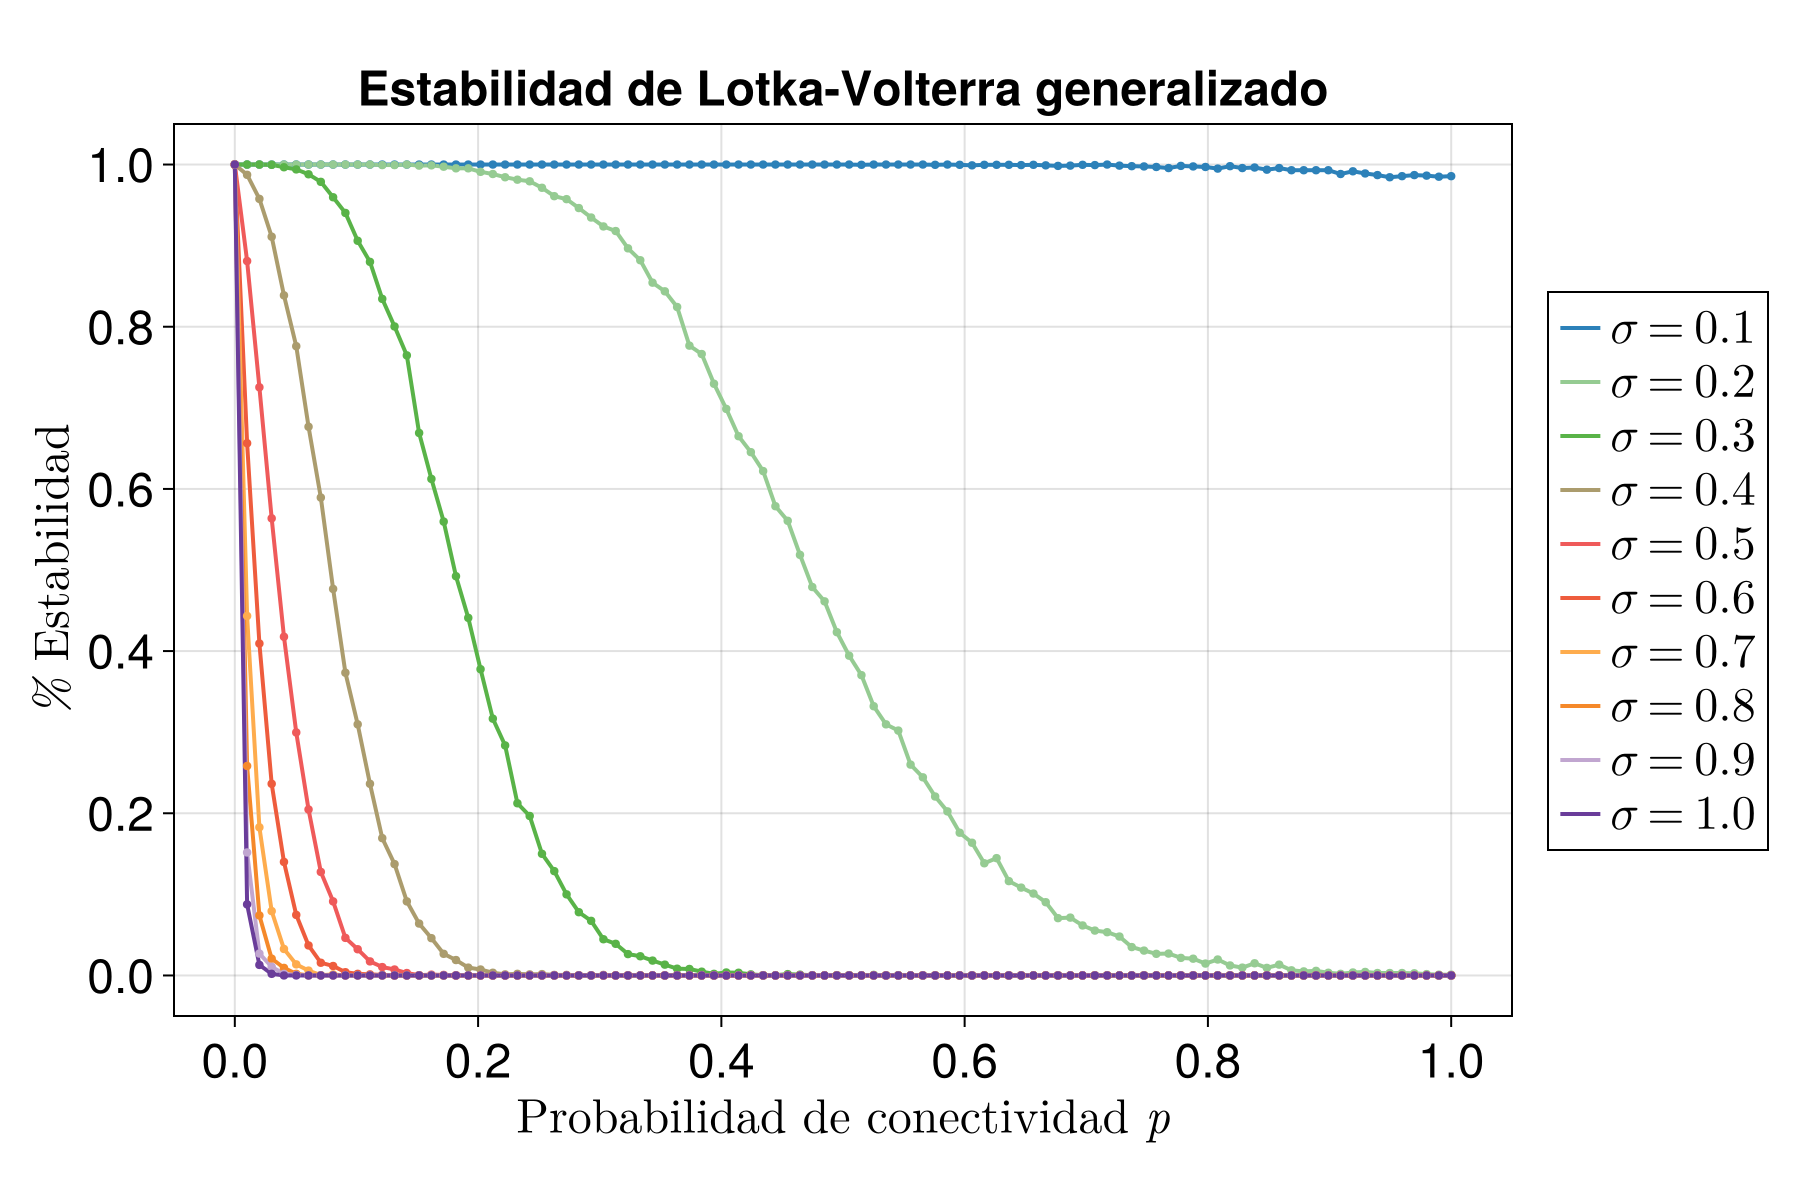
\includegraphics[scale=0.2]{../Imagenes/EstabilidadLKpLin.png}
	\caption{Transición dinámica del sistema de Lotka-Votlerra generalizado estructuralmente simétrico en función de la probabilidad de conectividad para $N=100$.}
	\label{fig:EstabilidadLKpLin}
\end{figure}

Un aspecto llamativo es que para $\sigma=0.2$ la región transitoria abarca una fracción considerable en el intervalo de $p$, lo que sugiere una disminución gradual de la probabilidad de estabilidad conforme aumenta la conectividad. Esto indica que, en éste régimen, pequeñas variaciones en $p$ producen cambios relativamente pequeños en la fracción de realizaciones estables a causa de la magnitud típica $\sigma$. Por tanto, en este caso la anchura del umbral crítico se difumina en función de $\sigma$. No obstante, en el límite cuando $N\to\infty$ se espera que el umbral crítico sea más abrupto, aún para magnitudes típicas pequeñas.
\\
\\
En contraste con magnitudes típicas mayores, se observa que el cambio de estabilidad ocurre en regiones tempranas de $p$ cuando $\sigma$ es grande y se desplaza hacia valores mayores de conectividad conforme $\sigma$ disminuye. Este comportamiento es consistente con el criterio de estabilidad de May y observado en la subsección \ref{sec:TransicionesMay}, el cual relaciona la pérdida de estabilidad con el crecimiento del radio espectral efectivo de la matriz Jacobiana. 
\\
\\
En la Figura \eqref{fig:EstabilidadLKpLog} se muestran las transiciones dinámicas en una escala $\log_{10}$ con el fin de resaltar las variaciones en las regiones tempranas del parámetro de control. La forma general de estas transiciones presenta similitudes cualitativas con las observadas en sistemas con soporte estructuralmente simétrico en el análisis clásico de May. Esto sugiere que ciertas propiedades dinámicas del sistema están fuertemente influenciadas por la estructura del soporte de la matriz de coeficientes $\Lambda$, particularmente en lo que respecta a la organización estadística de sus interacciones. 
\newpage
\begin{figure}[h!]
	\centering
	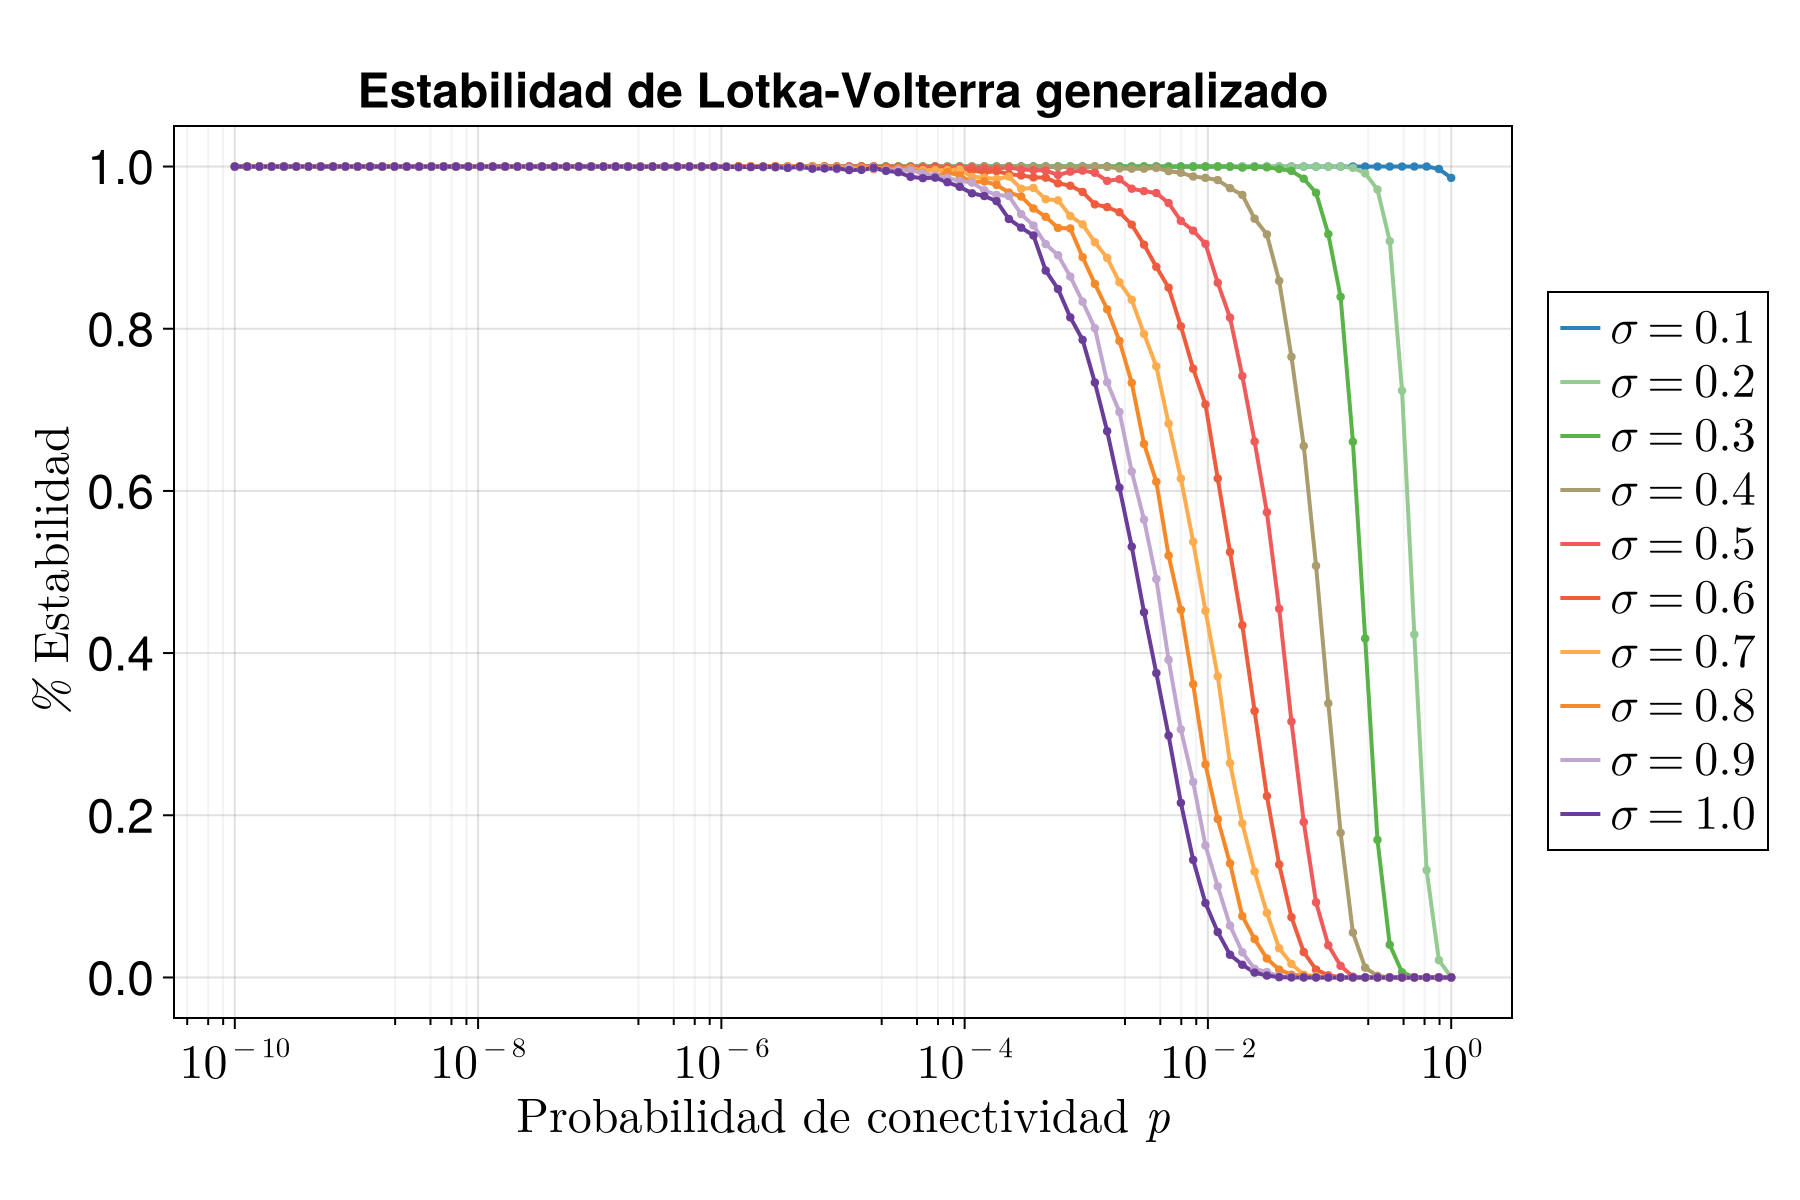
\includegraphics[scale=0.2]{../Imagenes/EstabilidadLKpLog}
	\caption{Transición dinámica del sistema de Lotka-Votlerra generalizado estructuralmente simétrico en función de la probabilidad con escala logarítmica para $N=100$.}
	\label{fig:EstabilidadLKpLog}
\end{figure}

Por otro lado, en la Figura \eqref{fig:ComparacionIncidenciasp} se muestra el contraste de las transiciones dinámicas entre sistemas en los que la matriz $\Lambda$ posee soporte estructuralmente simétrico y dirigido. El comportamiento observado es cualitativamente consistente con el contraste previamente analizado en los sistemas de May con diferentes estructuras de soporte.
\begin{figure}[h!]
	\centering
	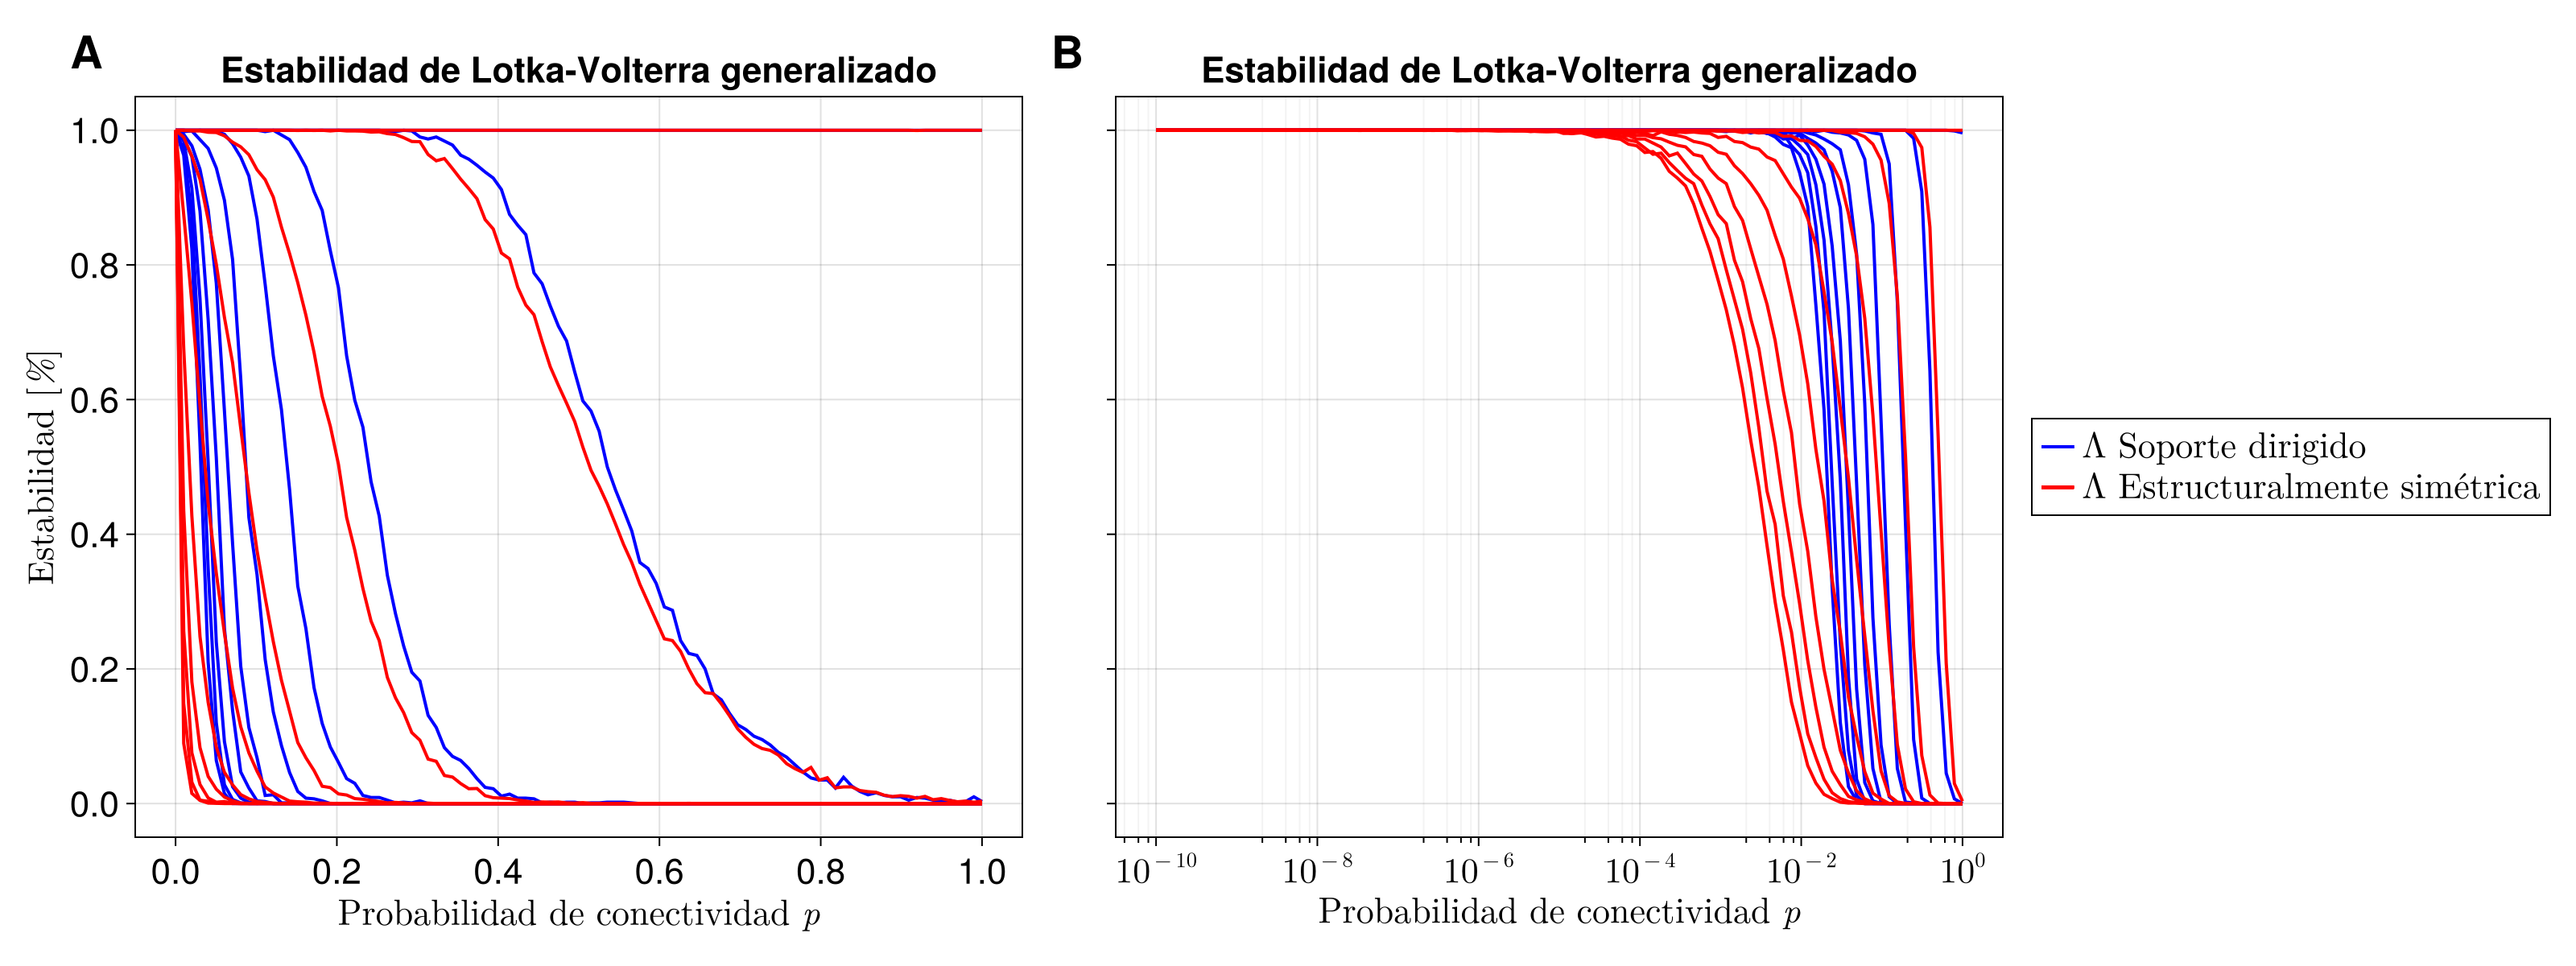
\includegraphics[scale=0.16]{../Imagenes/ComparacionIncidenciasp}
	\caption{Contraste de transiciones dinámicas entre sistemas de Lotka-Volterra generalizados con $\Lambda$ estructuralmente simétrica y de soporte dirigido.}
	\label{fig:ComparacionIncidenciasp}
\end{figure}

En particular, las transiciones asociadas a matrices con soporte dirigido presentan una pérdida de estabilidad más abrupta conforme aumenta la probabilidad $p$, mientras que los sistemas con soporte estructuralmente simétrico exhiben una región transitoria considerablemente más amplia. Esto refuerza que la estructura de soporte de $\Lambda$ influye de manera importante en las transiciones dinámicas del sistema, ya que la organización estadística de sus interacciones determina diferencias en la estructura espectral y, por lo tanto, en la probabilidad de estabilidad. En ese sentido, los sistemas estructuralmente simétricos muestran una transición más gradual, lo que sugiere una mayor robustez frente a variaciones del parámetro de control $p$. Una posible interpretación es que esta estructura favorece la aparición de configuraciones cercanas al borde de estabilidad, lo que ampliaría la región transitoria observada en las curvas de estabilidad.
\\
\\
En la Figura \eqref{fig:ComparacionLKMay} se muestran las desviaciones en la probabilidad de estabilidad entre el sistema de Lotka-Volterra generalizado de soporte dirigido y los sistemas aleatorios considerados en el análisis clásico de May. A pesar de las diferencias estructurales entre ambos sistemas, las caídas de estabilidad presentan un comportamiento cualitativamente similar. Esto sugiere que ciertas propiedades espectrales globales se conservan incluso después del reescalamiento multiplicativo inducido por las abundancias del equilibrio $X^*$ en la matriz Jacobiana $\mathcal{J}$.
\begin{figure}[h!]
	\centering
	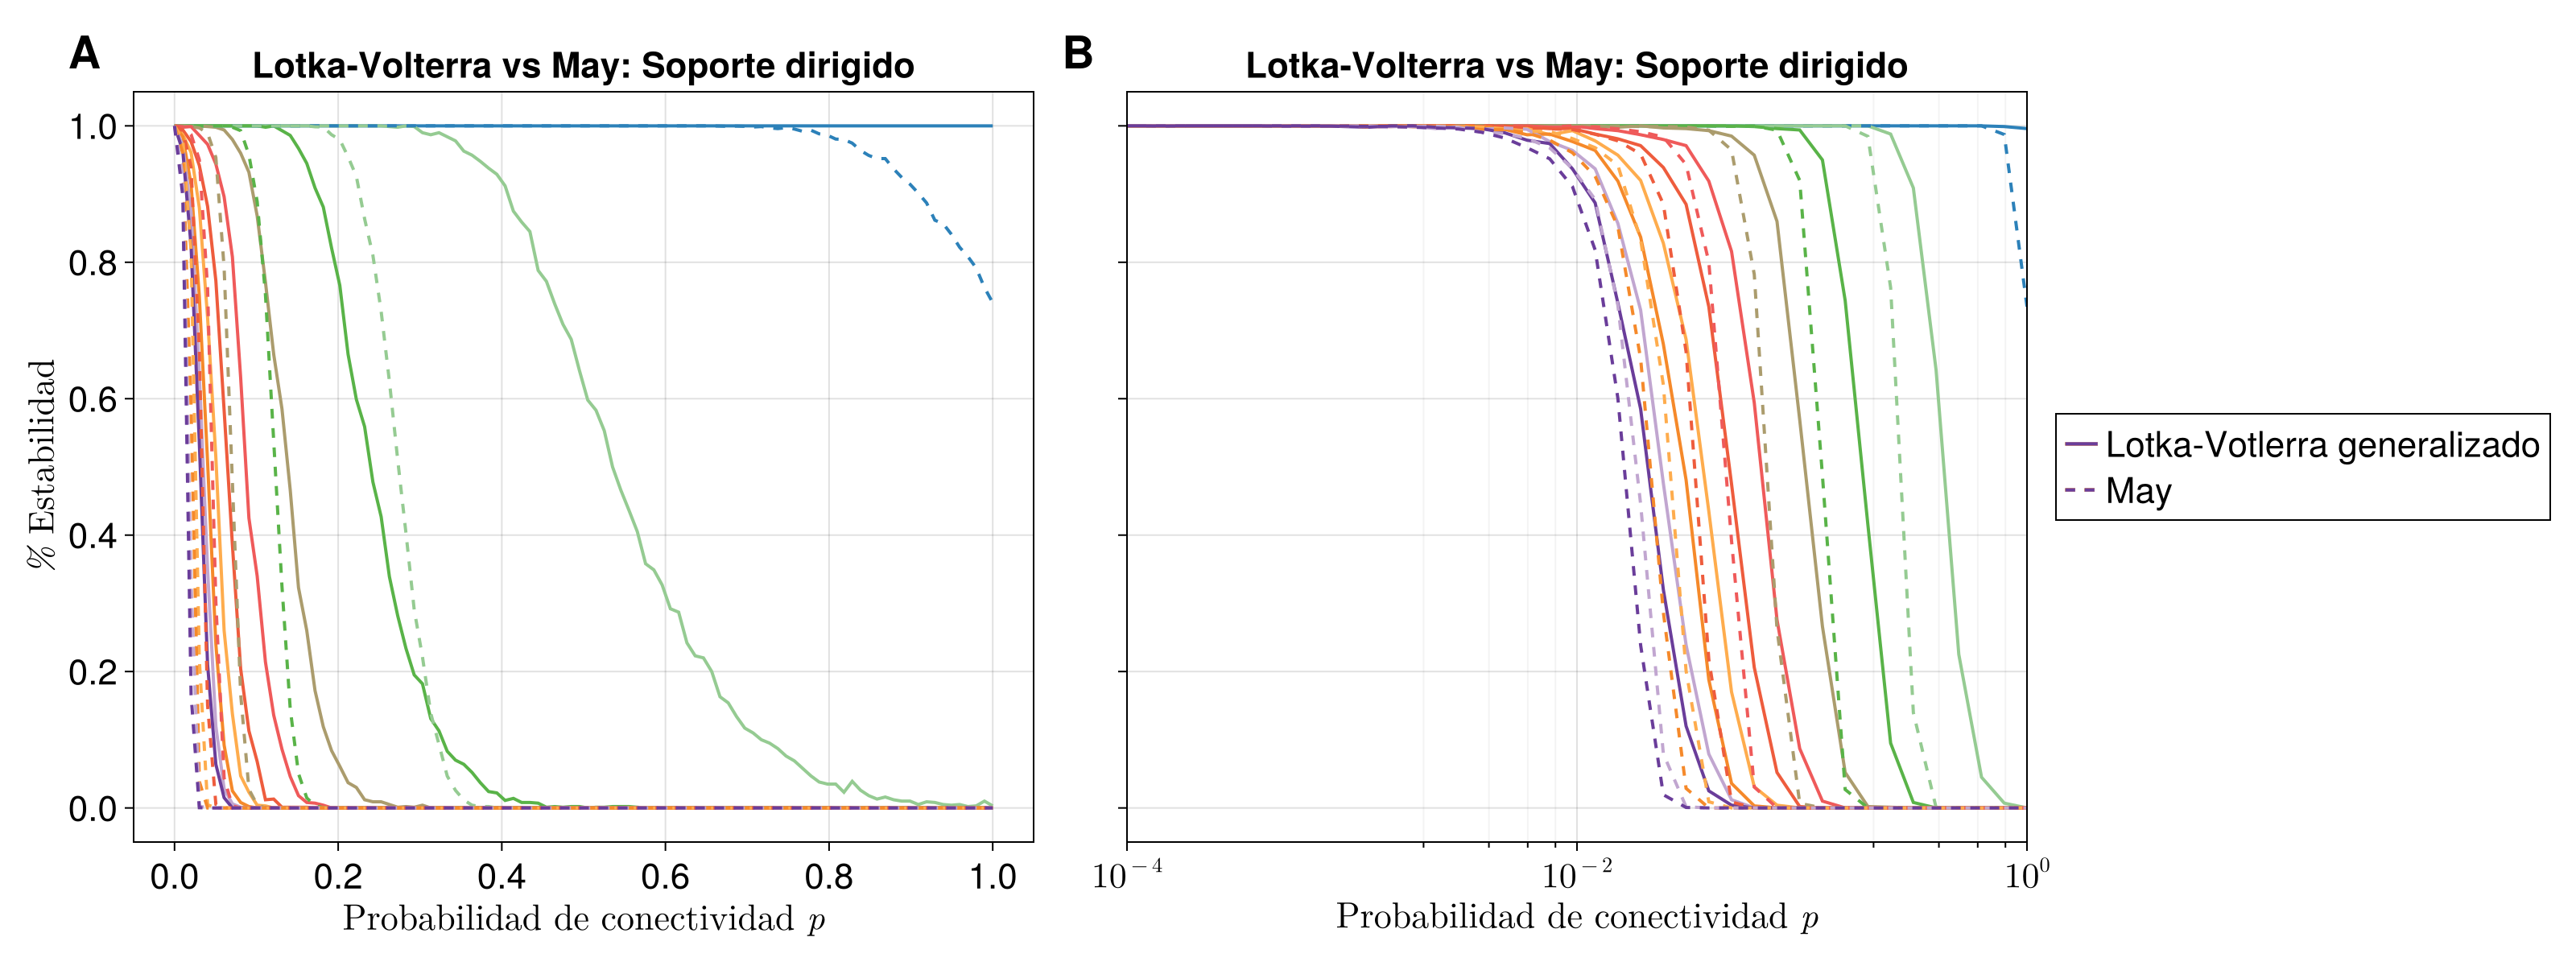
\includegraphics[scale=0.16]{../Imagenes/ComparacionLKMay.png}
	\caption{Contraste de transiciones dinámicas entre sistemas de Lotka-Volterra y May en función de $p$ con matrices de soporte dirigido.}
	\label{fig:ComparacionLKMay}
\end{figure}

Por otro lado, en la Figura \eqref{fig:ComparacionLKMayESim} se presenta de forma análoga el contraste entre sistemas Lotka-Volterra y sistemas de May cuando la matriz de interacciones posee soporte estructuralmente simétrico. En este caso, las desviaciones entre ambos modelos siguen siendo visibles; no obstante, las transiciones conservan una estructura cualitativamente similar. \\
\\
Este comportamiento sugiere que ciertas propiedades espectrales globales del sistema ---particularmente la anisotropía y la elongación del espectro en el plano complejo asociadas a este tipo de soporte--- continúan influyendo en la probabilidad de estabilidad, aún cuando la matriz Jacobiana efectiva esté modulada por el reescalamiento multiplicativo de las abundancias del equilibrio.
\newpage
\begin{figure}[h!]
	\centering
	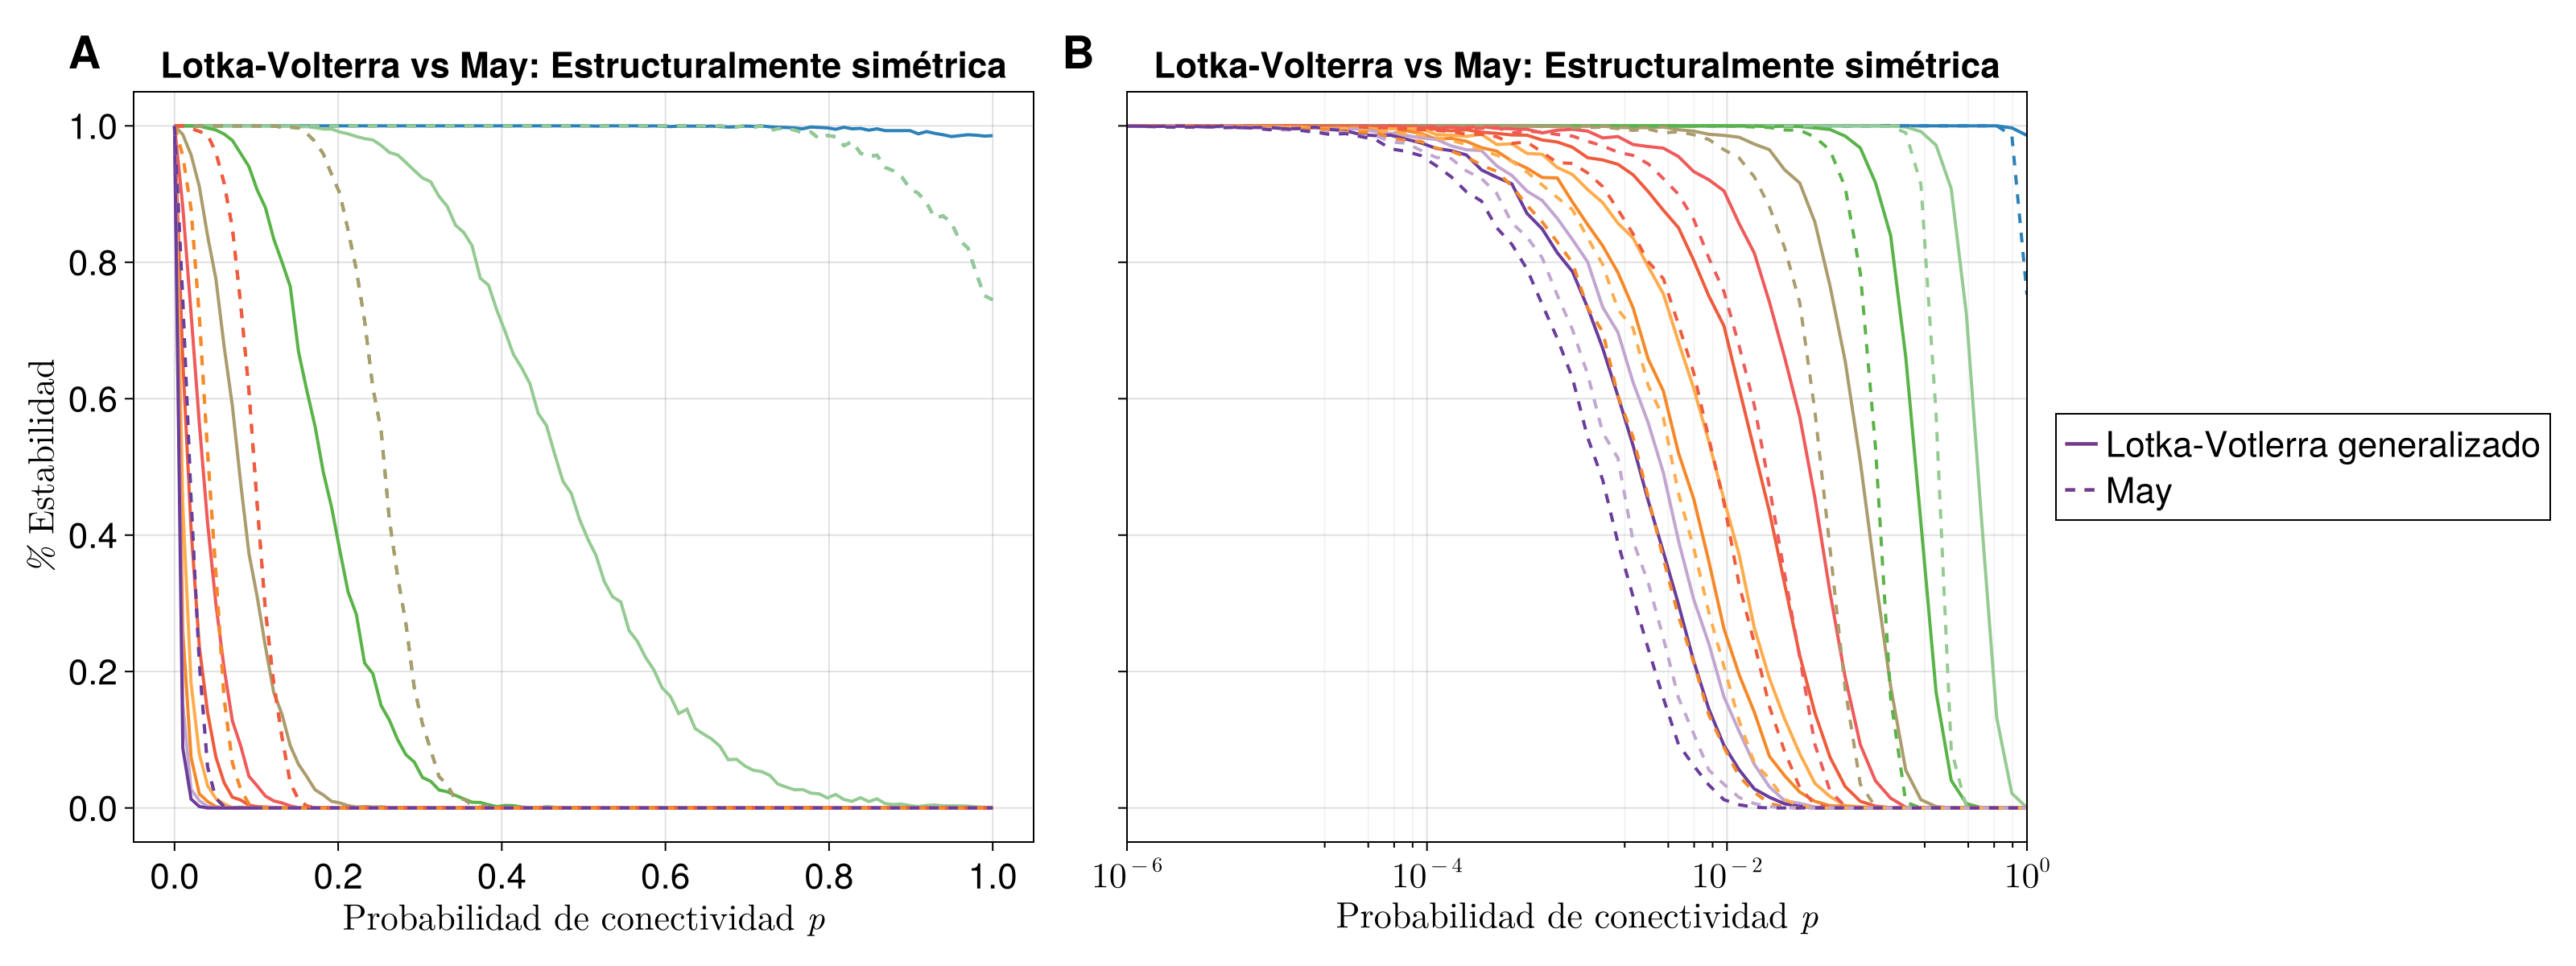
\includegraphics[scale=0.16]{../Imagenes/ComparacionLKMayESim.png}
	\caption{Contraste de transiciones dinámicas entre sistemas de Lotka-Volterra y May en función de $p$ con matrices estructuralmente simétricas.}
	\label{fig:ComparacionLKMayESim}
\end{figure}


\subsubsection*{En función de $\sigma$}

En el contexto de May, las transiciones en función de $\sigma$ se caracterizan por ser relativamente abruptas y están determinadas por el crecimiento del radio espectral de la matriz de interacciones. Asimismo, se observó que estas transiciones tienden a concentrarse conforme la conectividad aumenta. En este sentido, las diferencias dinámicas entre sistemas con soporte estructuralmente simétrico y dirigido se vuelven menos pronunciadas a medida que la red se vuelve más densa. Este comportamiento sugiere que, en regímenes de alta conectividad, la influencia específica de la estructura del soporte se atenúa, y el sistema tiende a aproximarse al comportamiento esperado para matrices aleatorias del tipo considerado en el análisis de May.\\
\\
En la Figura \eqref{fig:EstabilidadLKσLin} se muestra la caracterización de las transiciones dinámicas en función de $\sigma$ para sistemas estructuralmente simétricos. El comportamiento observado es análogo al descrito para matrices aleatorias de May, considerando las diferencias estructurales del soporte. En este caso, las transiciones se presentan de forma más definida para cada valor de $p$, lo que indica que las variaciones en $\sigma$ producen cambios de estabilidad más regulares que los observados en $p$. \\
\\
Asimismo, se observa que las interacciones tienden a concentrarse conforme la conectividad de la red aumenta. Este comportamiento es consistente con la tendencia previamente observada en sistemas densamente conectados, donde las diferencias entre configuraciones particulares se atenúan y el sistema muestra una transición de estabilidad más definida.
\newpage
\begin{figure}[h!]
	\centering
	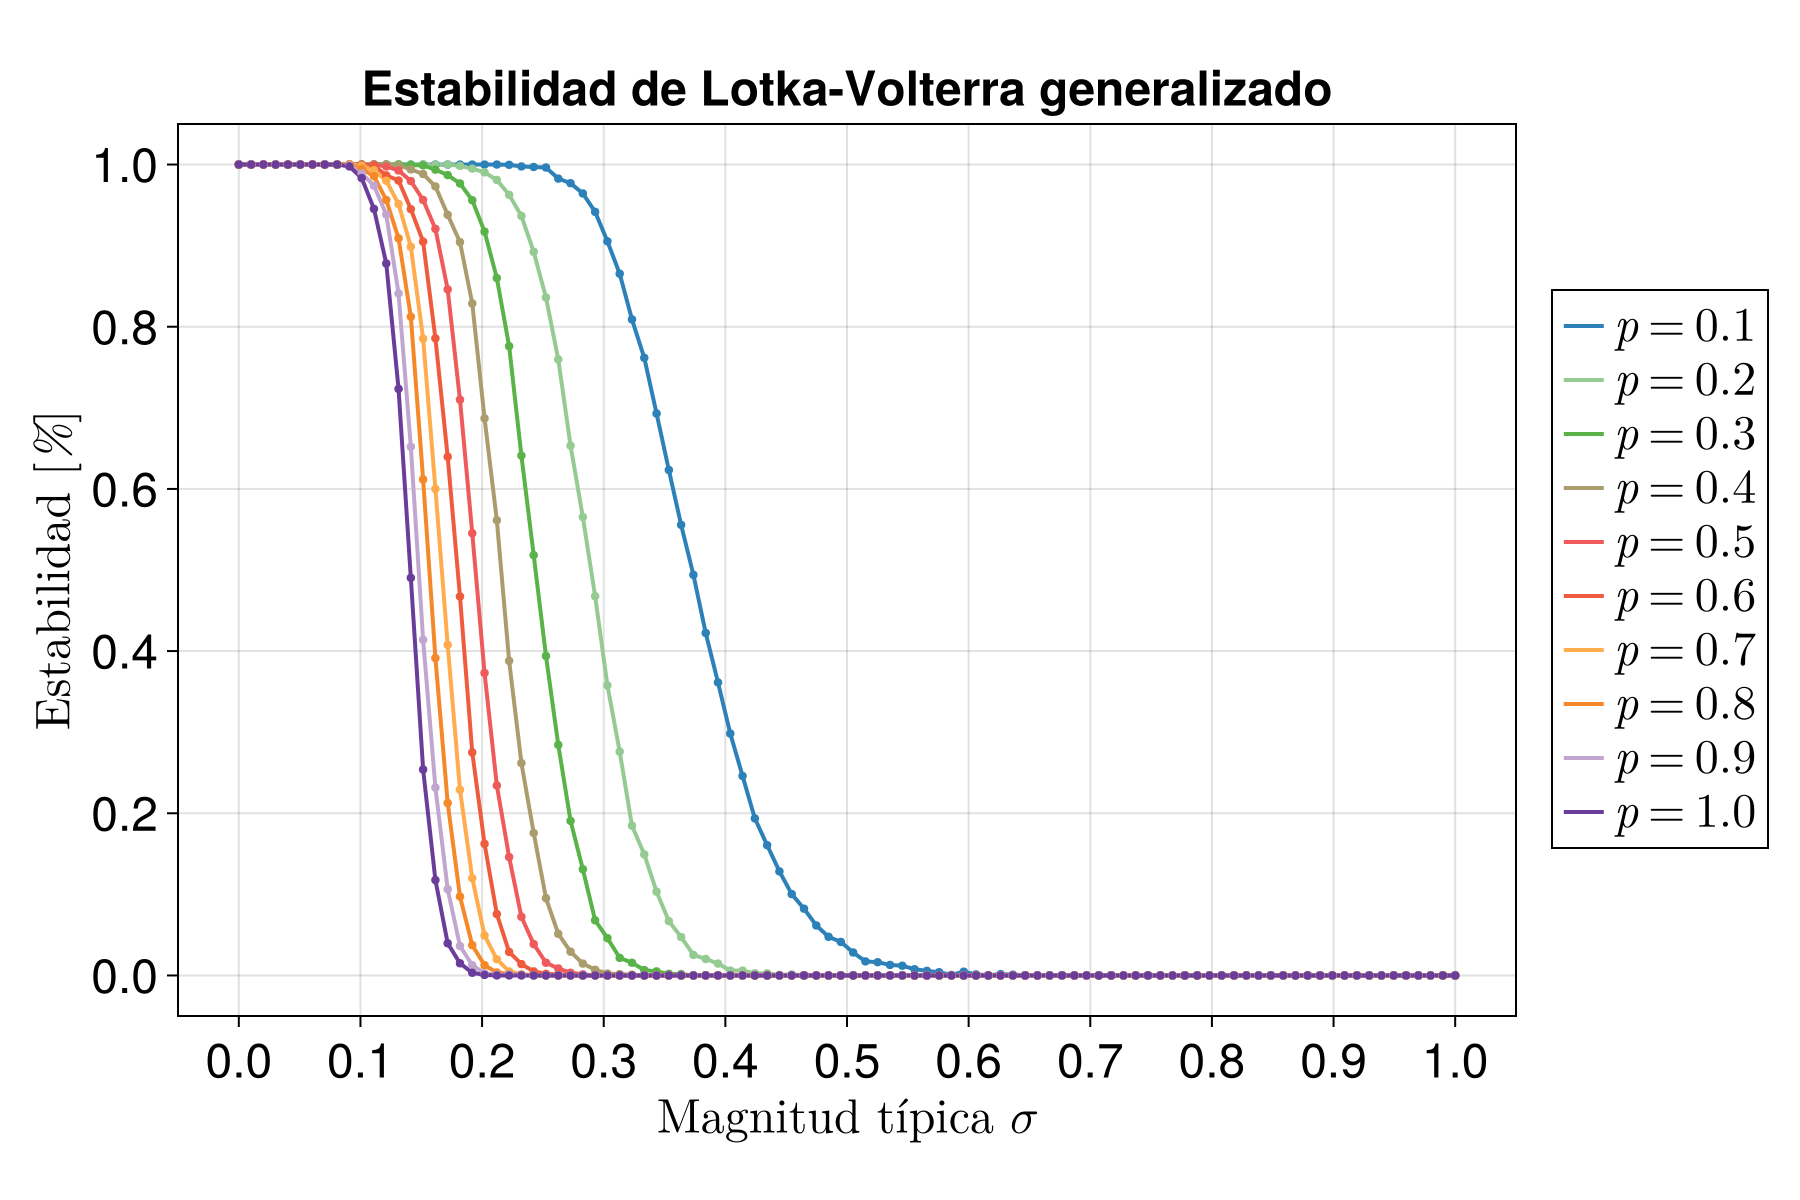
\includegraphics[scale=0.2]{../Imagenes/EstabilidadLKσLin}
	\caption{Transición dinámica del sistema de Lotka-Volterra generalizado estructuralmente simétrico en función de la magnitud típica para $N=100$.}
	\label{fig:EstabilidadLKσLin}
\end{figure}

Por otro lado, en la Figura \eqref{fig:ComparacionIncidenciasσ} se presenta el contraste en las transiciones del sistema Lotka-Volterra generalizado cuando la matriz de coeficientes $\Lambda$ posee soporte estructuralmente simétrico y dirigido. Se observa que las desviaciones entre ambos casos tienden a disminuir conforme la red se vuelve más conectada. Este comportamiento sugiere que la influencia específica del soporte estructuralmente simétrico se atenúa en regímenes de alta conectividad, donde la dinámica del sistema comienza a aproximarse al comportamiento esperado para matrices aleatorias densamente conectadas. 
\begin{figure}[h!]
	\centering
	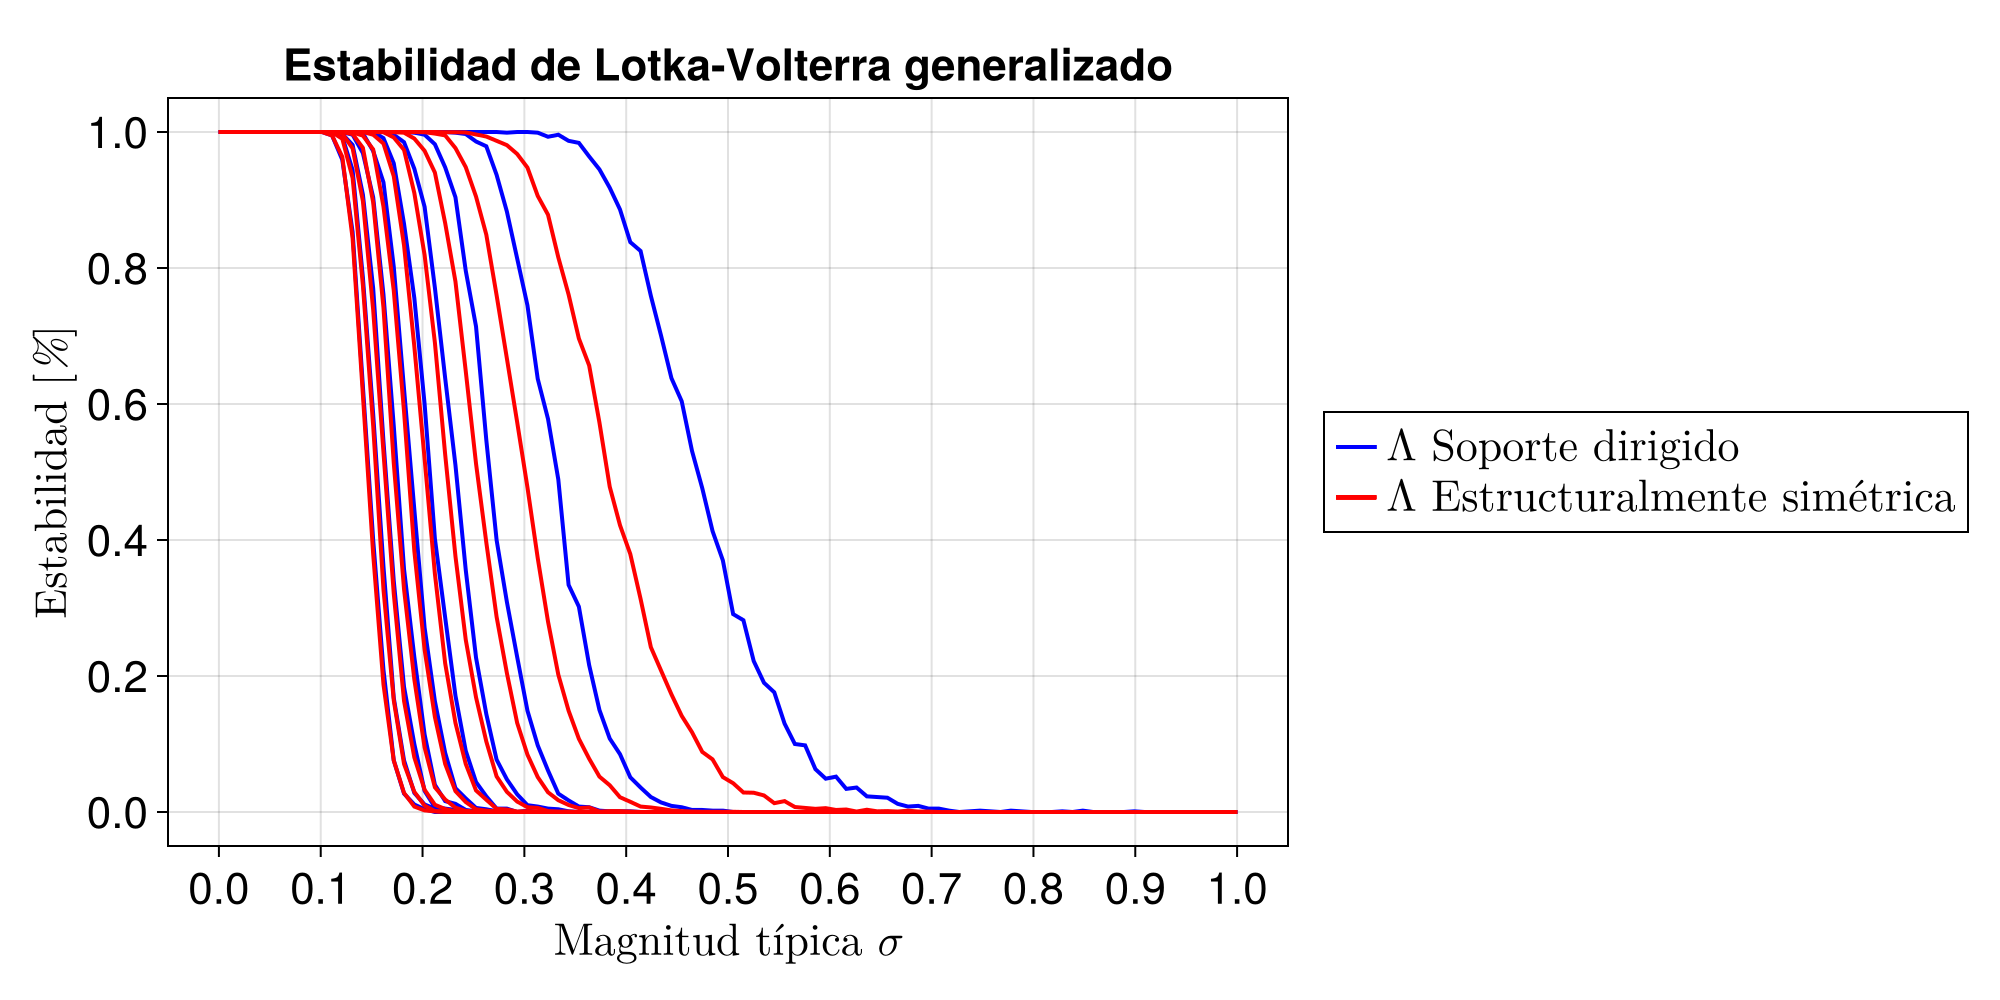
\includegraphics[scale=0.22]{../Imagenes/ComparacionIncidenciasσ}
	\caption{Comparación de la estabilidad entre sistemas de Lotka-Volterra generalizados en función de $\sigma$ con $\Lambda$ aleatoria y estructuralmente simétrica.}
	\label{fig:ComparacionIncidenciasσ}
\end{figure}

En consecuencia, las propiedades de estabilidad asociadas a las matrices Jacobianas en ambos casos tienden a volverse más similares a medida que aumenta la conectividad de la red. Finalmente, en la Figura \eqref{fig:ComparacionLKMayσ} se muestran las desviaciones del sistema de Lokta-Volterra generalizado con respecto a las matrices aleatorias consideradas en el análisis clásico de May, tanto para soportes estructuralmente simétricos como dirigidos. En ambos casos observa que las transiciones de estabilidad conservan una estructura cualitativamente similar, lo que sugiere que ciertas propiedades espectrales globales continúan influyendo en la dinámica aún cuando la matriz Jacobiana este modulada por las abundancias del equilibrio.

\begin{figure}[h!]
	\centering
	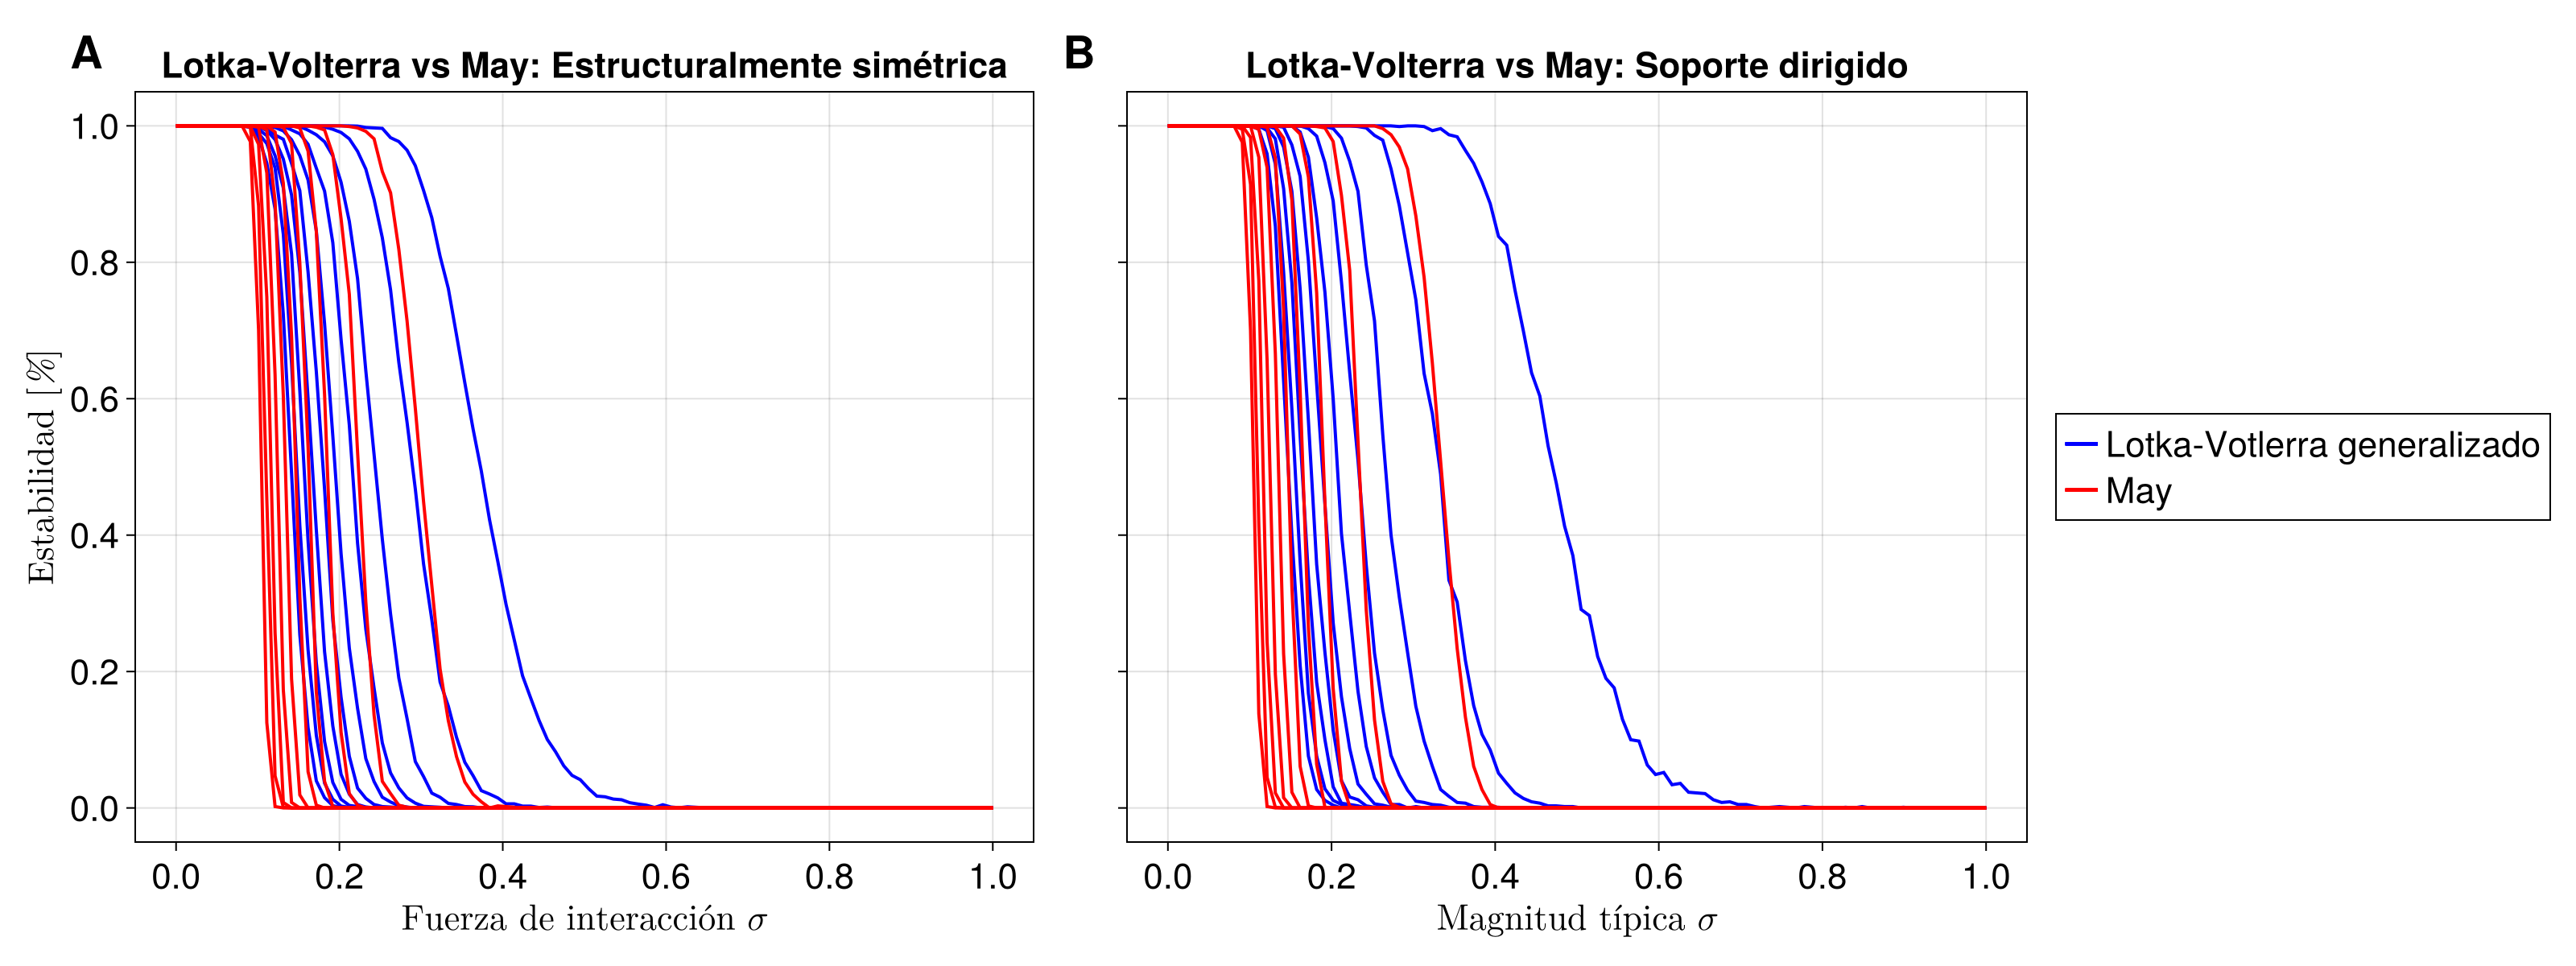
\includegraphics[scale=0.16]{../Imagenes/ComparacionLKMayσ}
	\caption{Comparación de la estabilidad entre sistemas de Lotka-Volterra y May en función de $\sigma$ con matrices aleatorias y estructuralmente simétricas.}
	\label{fig:ComparacionLKMayσ}
\end{figure}

En conjunto, las variaciones de los parámetros $p$ y $\sigma$ producen transiciones de estabilidad que guardan semejanza con las predichas en el marco clásico de May. Esto indica que el radio espectral de la matriz de interacciones sigue proporcionando una referencia útil para interpretar la estabilidad del sistema de Lotka-Volterra generalizado. Aunque la matriz Jacobiana se encuentre reescalada por las abundancias del equilibrio, la estructura estadística de la matriz $\Lambda$ continúa desempeñando un papel relevante en la organización espectral que determina la estabilidad del sistema.

\subsection{Para $N=50$}

\subsubsection*{En función de $p$}


Para este caso particular, así como para $N=25$, se empleó la misma metodología utilizada en el análisis para $N=100$. La única diferencia radica en el número de simulaciones realizadas por cada configuración  $(p,\sigma,N)$, tal como se muesrta en la Tabla \eqref{tab:SimulacionesTransicion}. En estos sistemas de menor dimensión se requiere un mayor número de realizaciones para mitigar el ruido estadístico en la estimación de la probabilidad de estabilidad. \\
\\
En la Figura \eqref{fig:EstabilidadLKp50} se presentan las transiciones dinámicas con soporte estructuralmente simétrico en función de $p$. Se observa percibir que las regiones transitorias son más amplias en comparación con el caso $N=100$, lo que indica que pequeñas variaciones en $p$ producen cambios aún más graduales en la probabilidad de estabilidad.  En este sentido, el comportamiento observado para $\sigma=0.3$ resulta cualitativamente similar al caso $\sigma=0.2$ cuando $N=100$
\begin{figure}[h!]
	\centering
	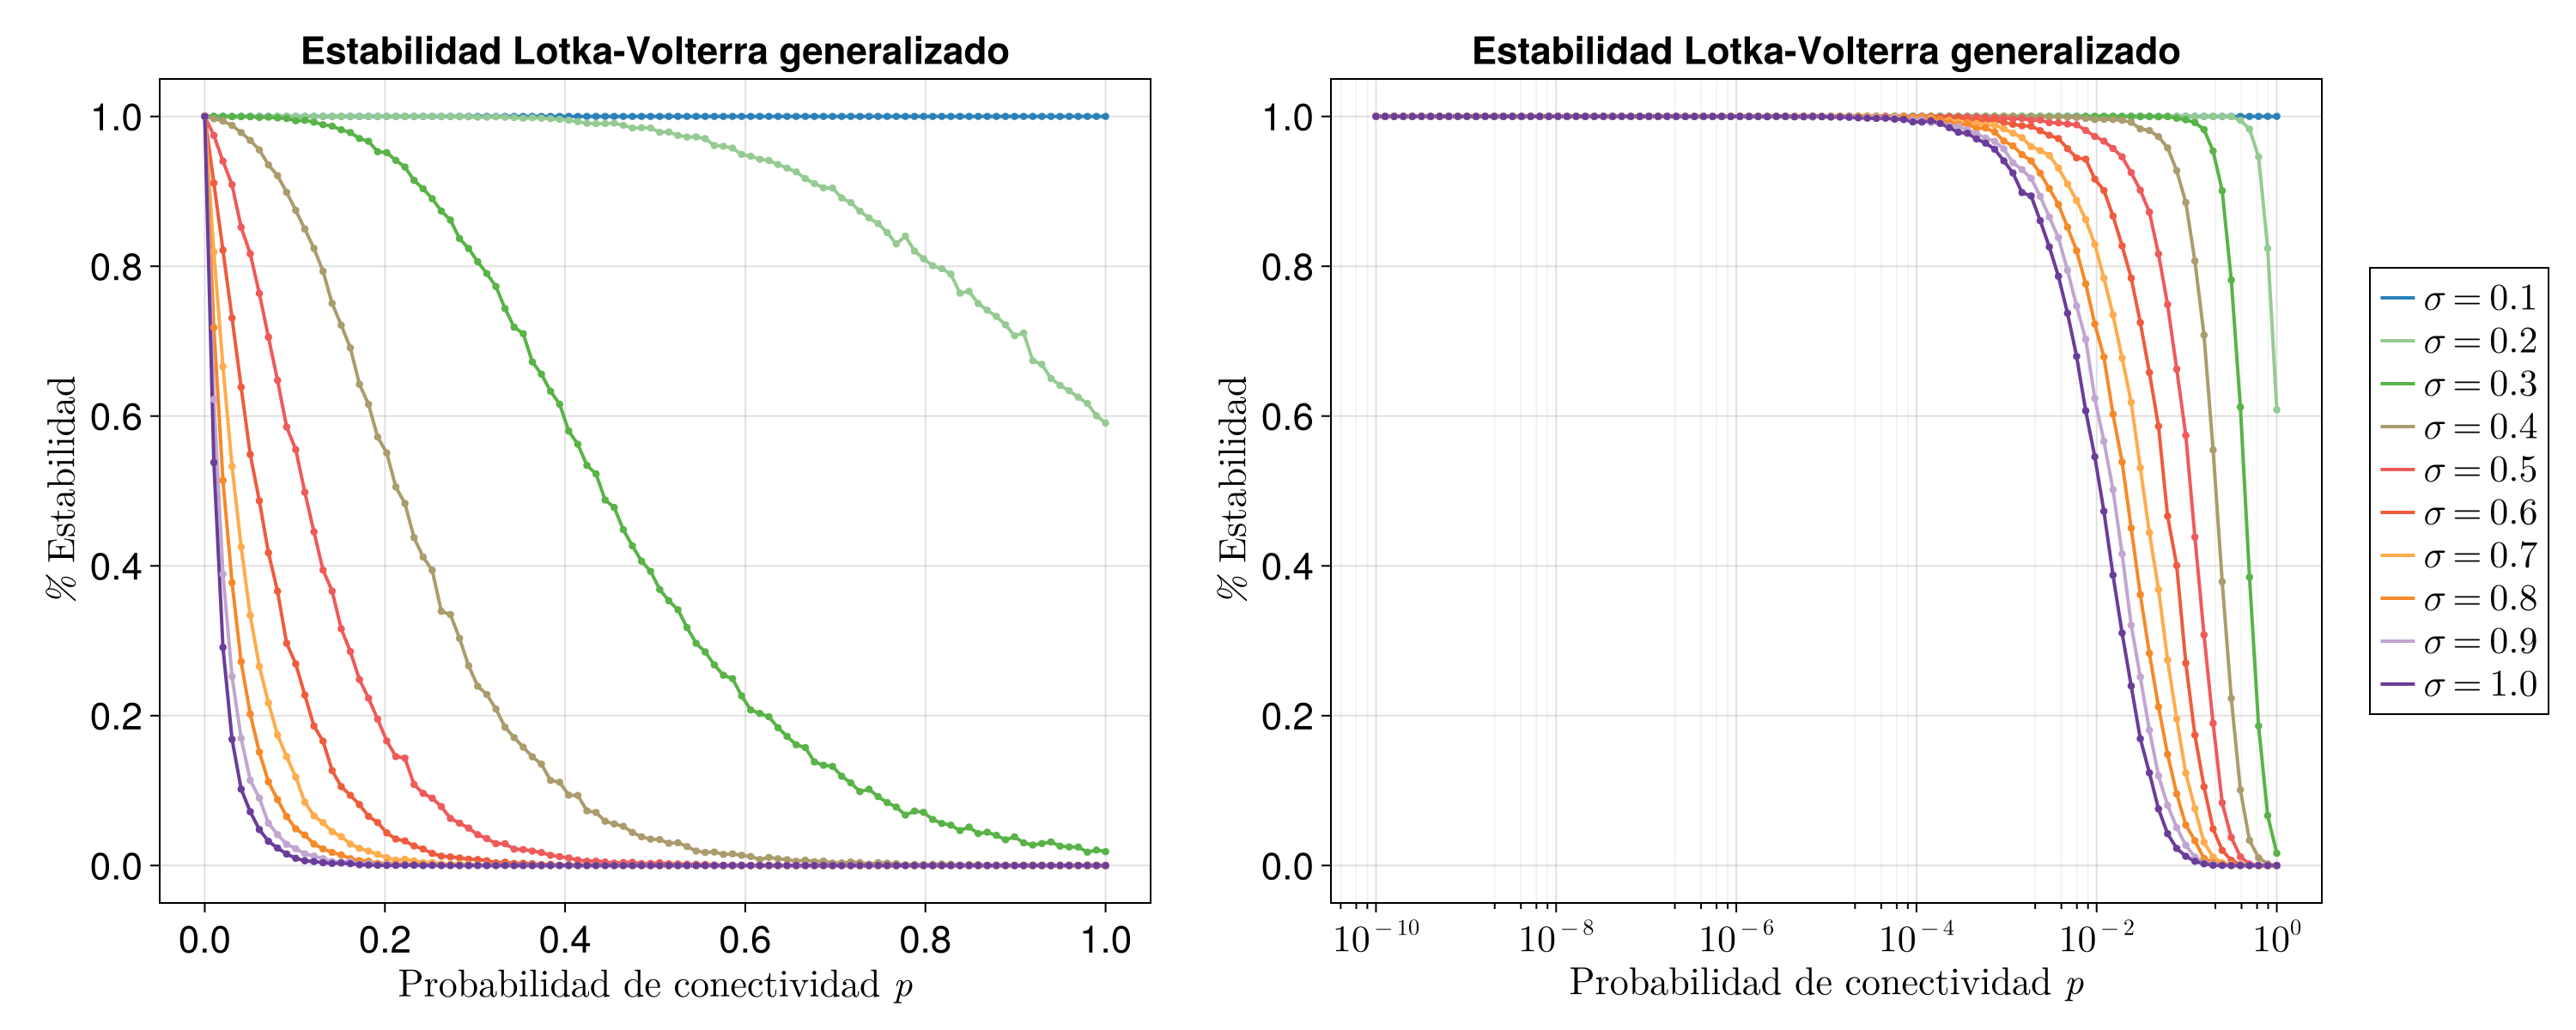
\includegraphics[scale=0.16]{../Imagenes/EstabilidadLKp50}
	\caption{Transición dinámica del Sistema de Lotka-Volterra generalizado estructuralmente simétrico en función de la probabilidad de conectividad para $N=50$.}
	\label{fig:EstabilidadLKp50}
\end{figure}

Sin embargo, aún para este tamaño del sistema se conserva la tendencia a que las transiciones ocurran más temprano conforme aumenta la magnitud $\sigma$, aunque en términos absolutos estas se encuentren desplazadas hacia valores mayores de $p$ con respecto del caso $N=100$. De manera preliminar, estas observaciones sugieren que, para los rangos de parámetros considerados, los sistemas de menor dimensión presentan una mayor probabilidad de estabilidad.

\subsubsection*{En función de $\sigma$}

De manera análoga en la Figura \eqref{fig:EstabilidadLKσ50}, las transiciones en $\sigma$ de sistemas con soporte estructuralmente simétrico también se presentan de forma más gradual en comparación con el caso $N=100$. No obstante, se conserva la tendencia a que estas se concentren conforme aumente la conectividad de la red.
\begin{figure}[h!]
	\centering
	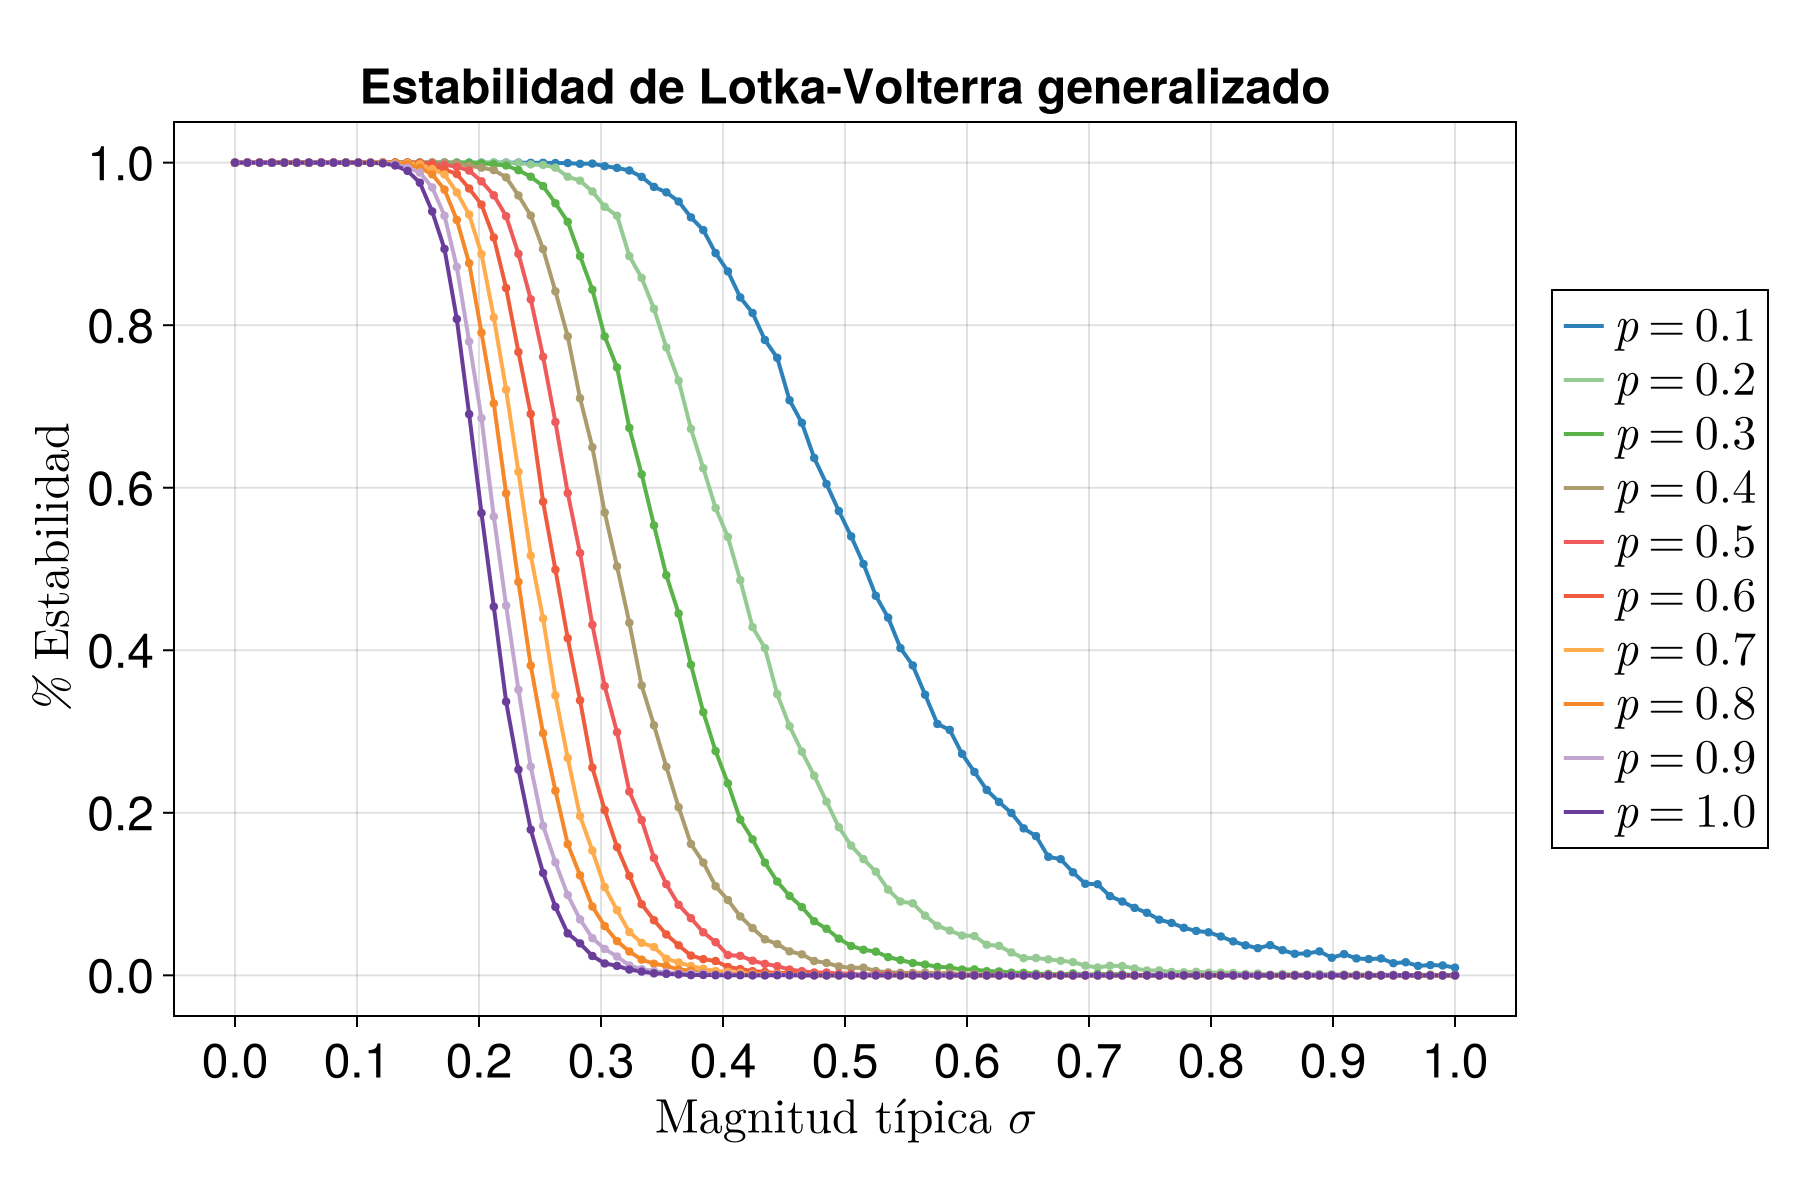
\includegraphics[scale=0.2]{../Imagenes/EstabilidadLKσ50}
	\caption{Transición dinámica del sistema de Lotka-Volterra generalizado estructuralmente simétrico en función de la fuerza de interacción para $N=50$.}
	\label{fig:EstabilidadLKσ50}
\end{figure}
\newpage
\subsection{Para $N=25$}

\subsubsection*{En función de $p$}

Finalmente, en la Figura \eqref{fig:EstabilidadLKp25} se muestran las transiciones dinámicas con soporte estructuralmente simétrico en función de $p$ para $N=25$. En esta caso las regiones transitorias son aún más amplias que en los sistemas de mayor dimensión, lo que indica que las variaciones en $p$ producen cambios más graduales en la probabilidad de estabilidad. Esto confirma que el tamaño del sistema también influye de manera relevante en la organización de las transiciones dinámicas.

\begin{figure}[h!]
	\centering
	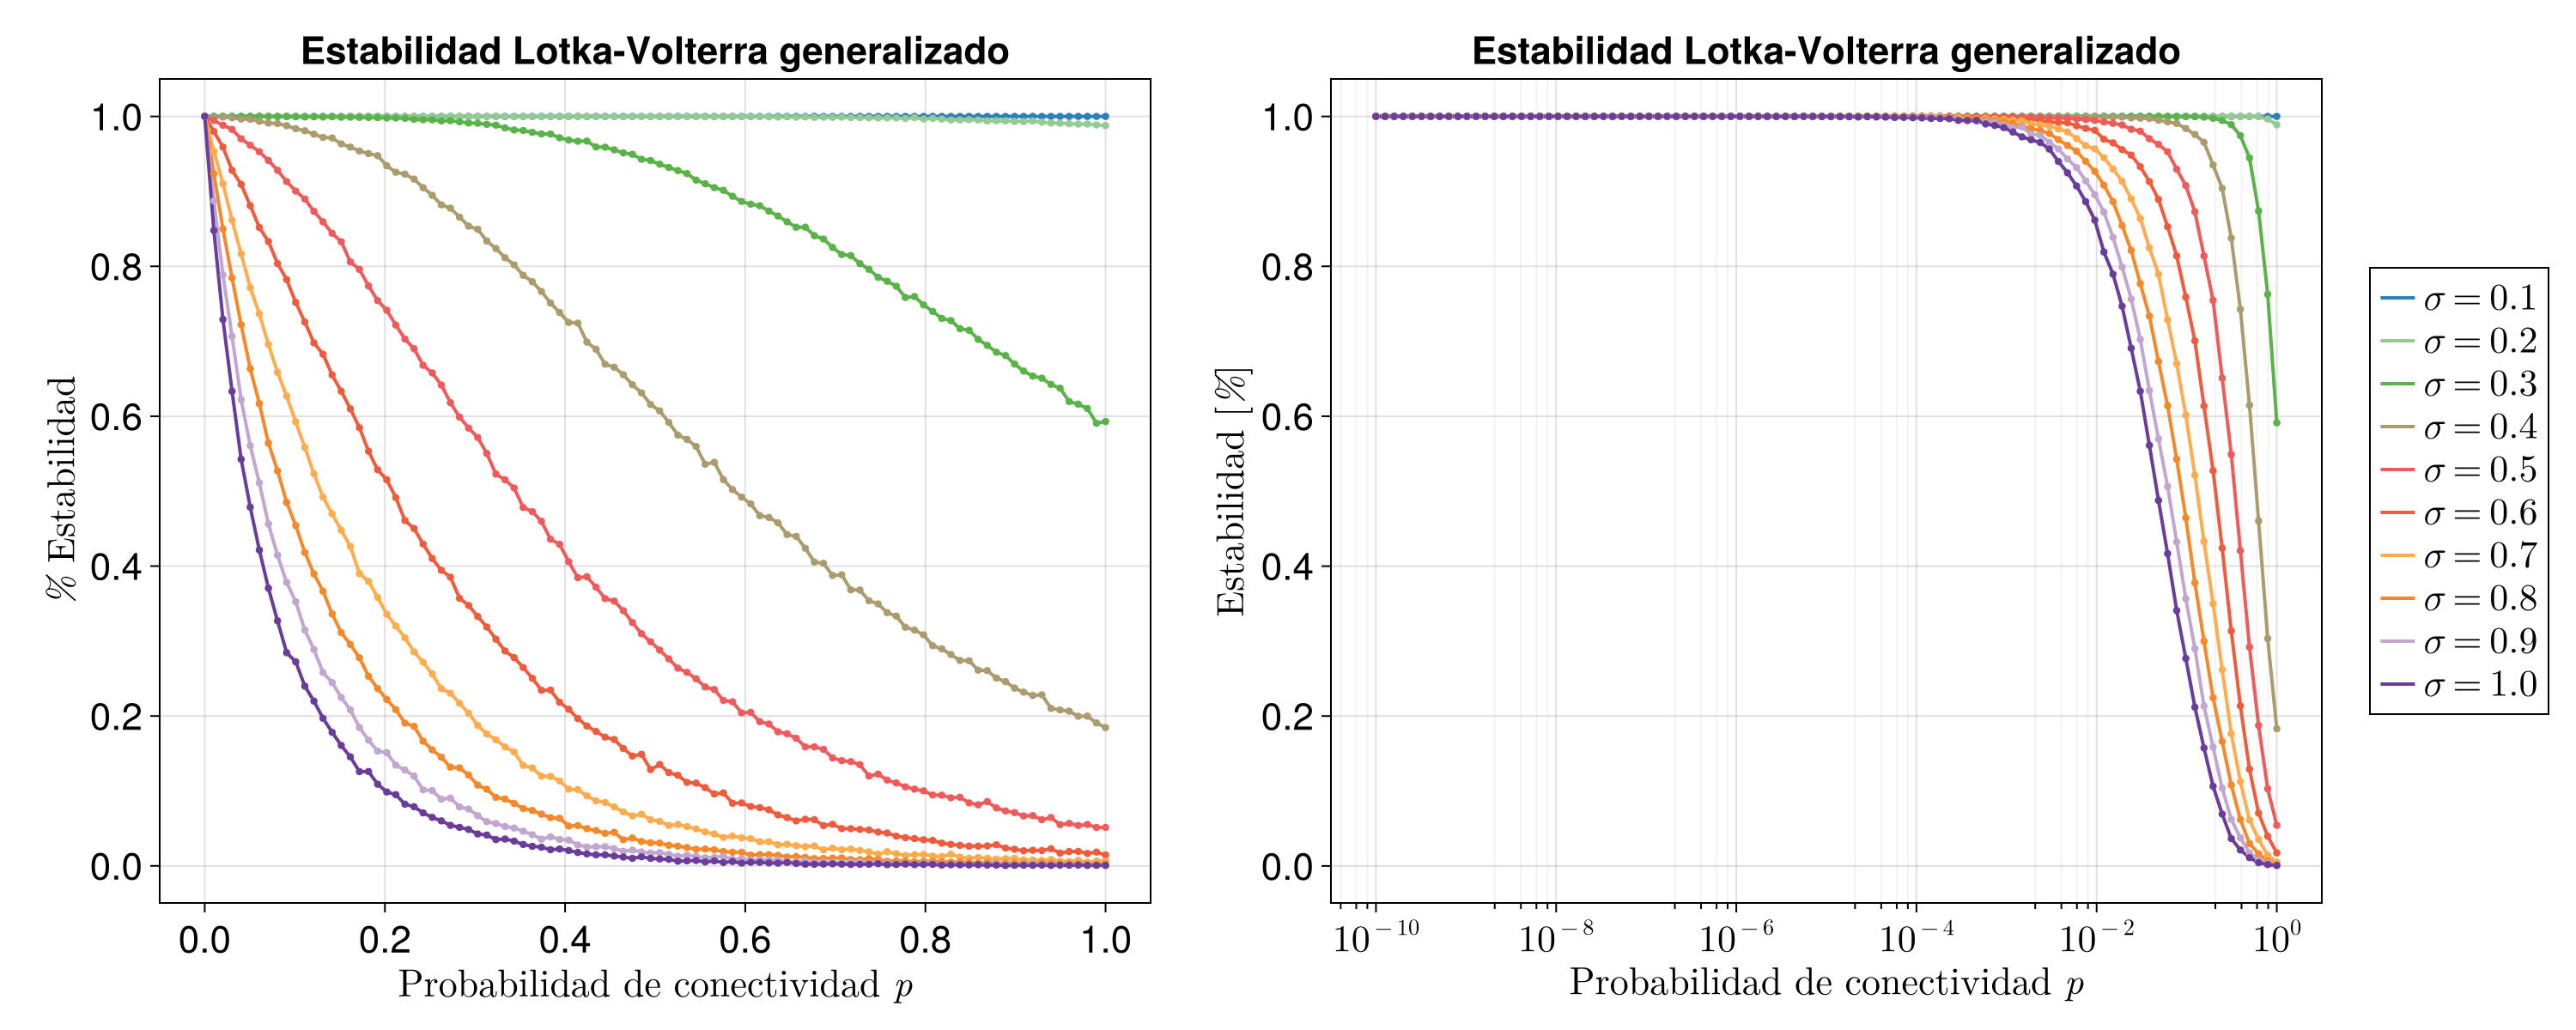
\includegraphics[scale=0.16]{../Imagenes/EstabilidadLKp25}
	\caption{Transición dinámica del sistema de Lotka-Volterra generalizado en función de la probabilidad de conectividad para $N=25$.}
	\label{fig:EstabilidadLKp25}
\end{figure}

\subsubsection*{En función de $\sigma$}

De manera análoga, en la Figura \eqref{fig:EstabilidadLKσ25} se presentan las transiciones en función de $\sigma$, las cuales muestran un comportamieinto cualitativamente similar al observado en los casos de mayor dimensión, aunque con regiones transitorias más amplias.
\begin{figure}[h!]
	\centering
	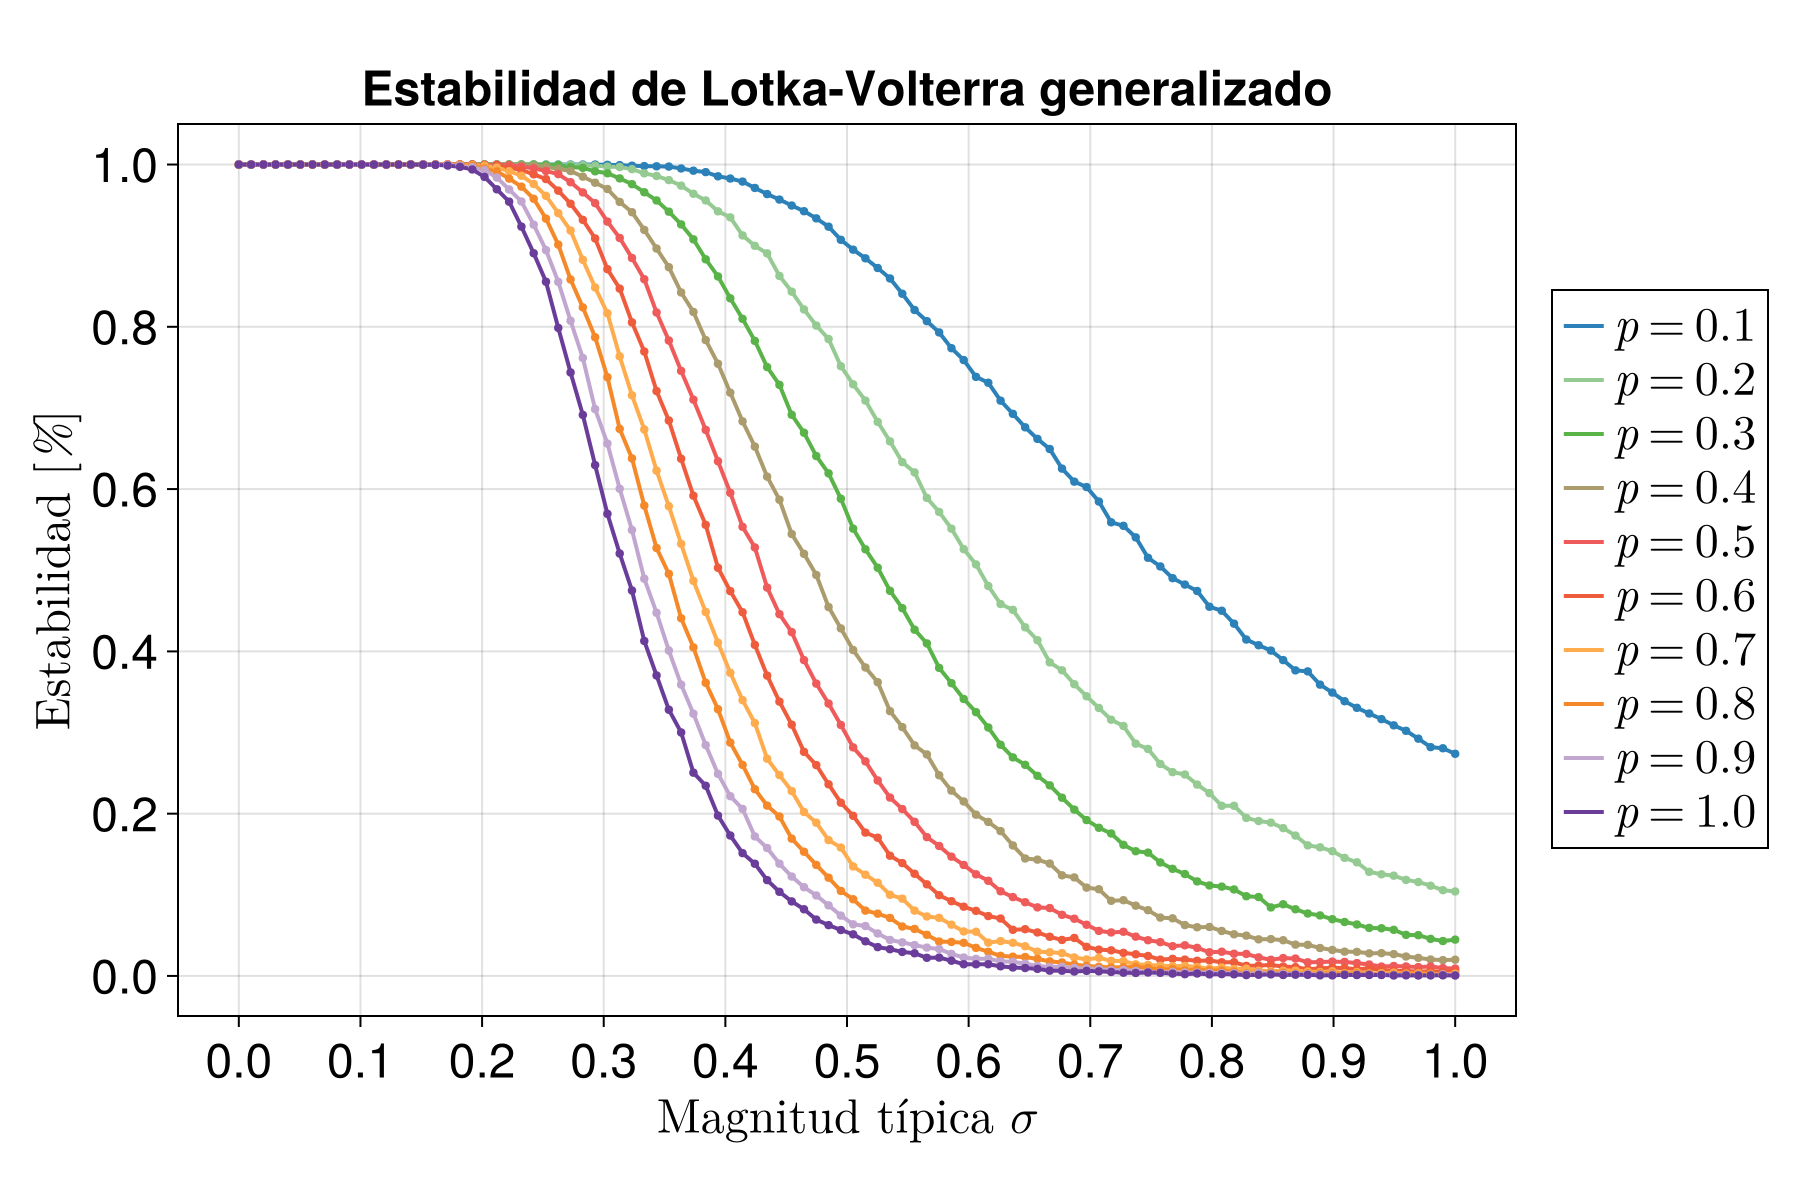
\includegraphics[scale=0.2]{../Imagenes/EstabilidadLKσ25}
	\caption{Transición dinámica del sistema de Lotka-Votlerra generalizado en función de la fuerza de interacción para $N=25$.}
	\label{fig:EstabilidadLKσ25}
\end{figure}

En conjunto, estos resultados sugieren que los sistemas de menor dimensión requieren interacciones de mayor magnitud para abandonar el régimen de estabilidad. De forma inductiva, esto apunta a que conforme el tamaño del sistema aumenta, las transiciones de estabilidad tienden a volverse más abruptas y a ocurrir para valores más pequeños de la magnitud típica de las interacciones.

\section{Indicador espectral para la transición de estabilidad}


Hasta este punto se ha obtenido una caracterización detallada de las transiciones dinámicas del sistema Lokta-Volterra generalizado. En particular, los resultados muestran una tendencia a preservar ciertas características estructurales que se originan de la matriz de coeficientes de interacción $\Lambda$ y que se reflejan posteriormente en la matriz Jacobiana. Asimismo, se ha observado que las transiciones de estabilidad en sistemas Lotka-Volterra con soporte estructuralmente simétrico y dirigido presentan semejanzas cualitativas con las transiciones predichas por el marco clásico de matrices aleatorias de May, aún cuando la Jacobiana efectiva se encuentre modulada por el reescalamiento multiplicativo de las abundancias del equilibrio.
\newpage
Estas observaciones sugieren que la estabilidad del sistema de Lotka-Volterra generalizado puede interpretarse, al menos de forma aproximada, a partir del radio espectral de la matriz de interacciones y del criterio de estabilidad de May. En este sentido, resulta natural considerar el radio espectral como un punto de partida estructural, al cual pueden incorporarse correcciones que tomen en cuenta las desviaciones anisotrópicas que emergen del espectro de la matriz Jacobiana. Bajo esta perspectiva, es posible proponer un indicador heurístico que permita aproximar el umbral de transición de estabilidad en estos sistemas.

\subsection{Borde de estabilidad para $N=2$}

Como se ha mencionado anteriormente, una forma de aproximar el umbral de estabilidad del sistema consiste en analizar la estructura espectral de la matriz $\Lambda$. En  particular, sus valores propios proporcionan una escala natural que influye en la magnitud de las abundancias del equilibrio $X^*$. Cuando algún valor propio de $\Lambda$ se aproxima a cero, $\Lambda$ se vuelve cercana a singular, lo que puede inducir grandes variaciones en las abundancias del equilibrio $X^*$. En estas condiciones, el sistema tiende a situarse cerca del borde de estabilidad, ya que la estructura de la Jacobiana puede volverse altamente sensible a pequeñas perturbaciones en la matriz $\Lambda$.\\
\\
En este contexto, el caso particular $N=2$ en un sistema con soporte estructuralmente simétrico permite visualizar de manera directa este mecanismo y proporciona una intuición útil sobre la relación entre la estructura espectral de $\Lambda$ y el umbral de estabilidad. Para interacciones de cooperación
\begin{wrapfigure}{l}{0.5 \textwidth} \vspace{-20pt} \begin{center}
		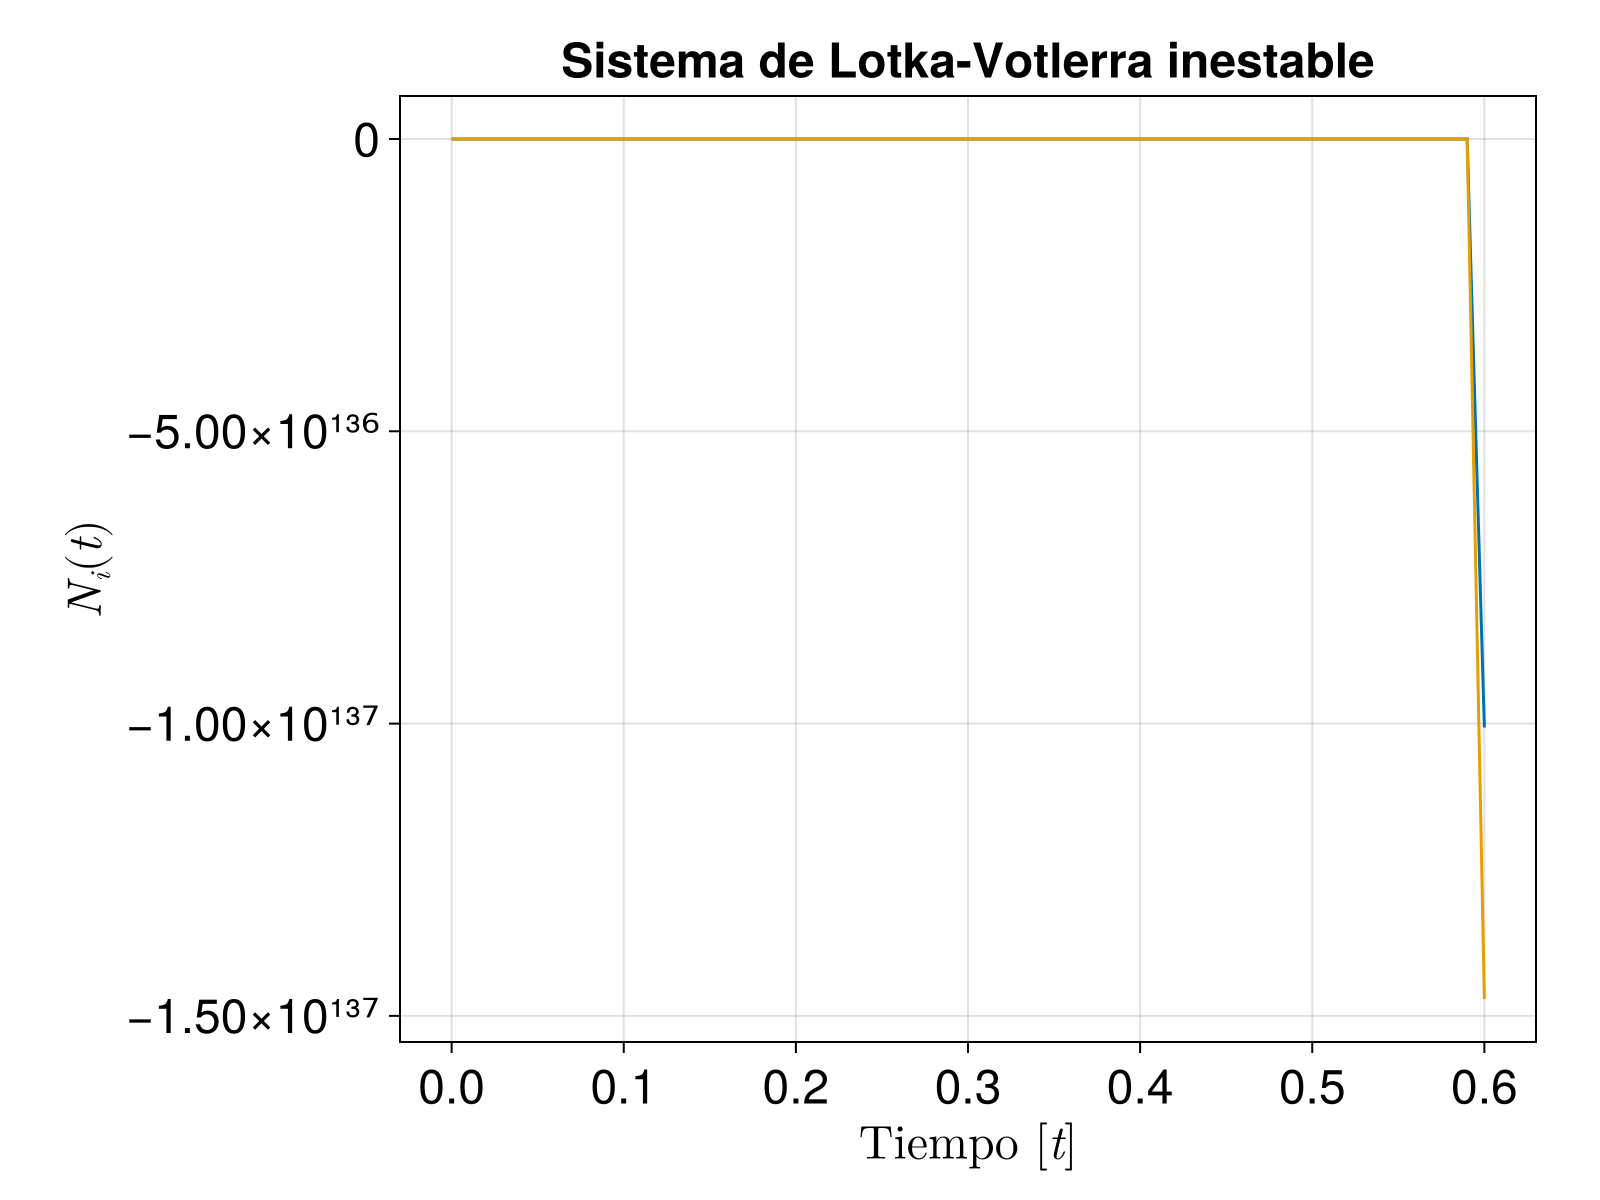
\includegraphics[scale=0.135]{../Imagenes/Heuristico}
	\end{center}
	\vspace{-20pt} 
	\caption{Sistema $N=2$ inestable con interacciones $\alpha_{12}\alpha_{21}>1$.}
	\vspace{20pt}
	\label{fig:Heuristico}
\end{wrapfigure}
en $\Lambda$ $(--)$, la estabilidad del sistema se encuentra directamente relacionada con la magnitud del ciclo de interacción entre ambas especies. En particular, se obtiene la condición
\begin{equation}\label{eqn:relacionHeuristica}
	\alpha_{12}\alpha_{21} < 1
\end{equation}
La cual garantiza que el sistema se mantiene en el régimen de estabilidad. En este caso, el determinante de coeficientes de interacción esta dado por
$$\det(\Lambda)=1-\alpha_{12}\alpha_{21}$$
Por lo tanto, la estabilidad del sistema se encuentra asociada al signo del determinante. Cuando $\det(\Lambda)>0$, ambos valores propios permanecen positivos y el sistema se mantiene estable. En contraste, cuando $\alpha_{12}\alpha_{21}>1$, el determinante se vuelve negativo y el sistema presenta un valor propio negativo, lo que conduce a la pérdida de estabilidad\footnote{En este caso, los valores propios son $\lambda_{\pm}=1\pm\sqrt{\alpha_{12}\alpha_{21}}$.}.

\begin{wrapfigure}{r}{0.5 \textwidth} \vspace{-30pt} \begin{center}
		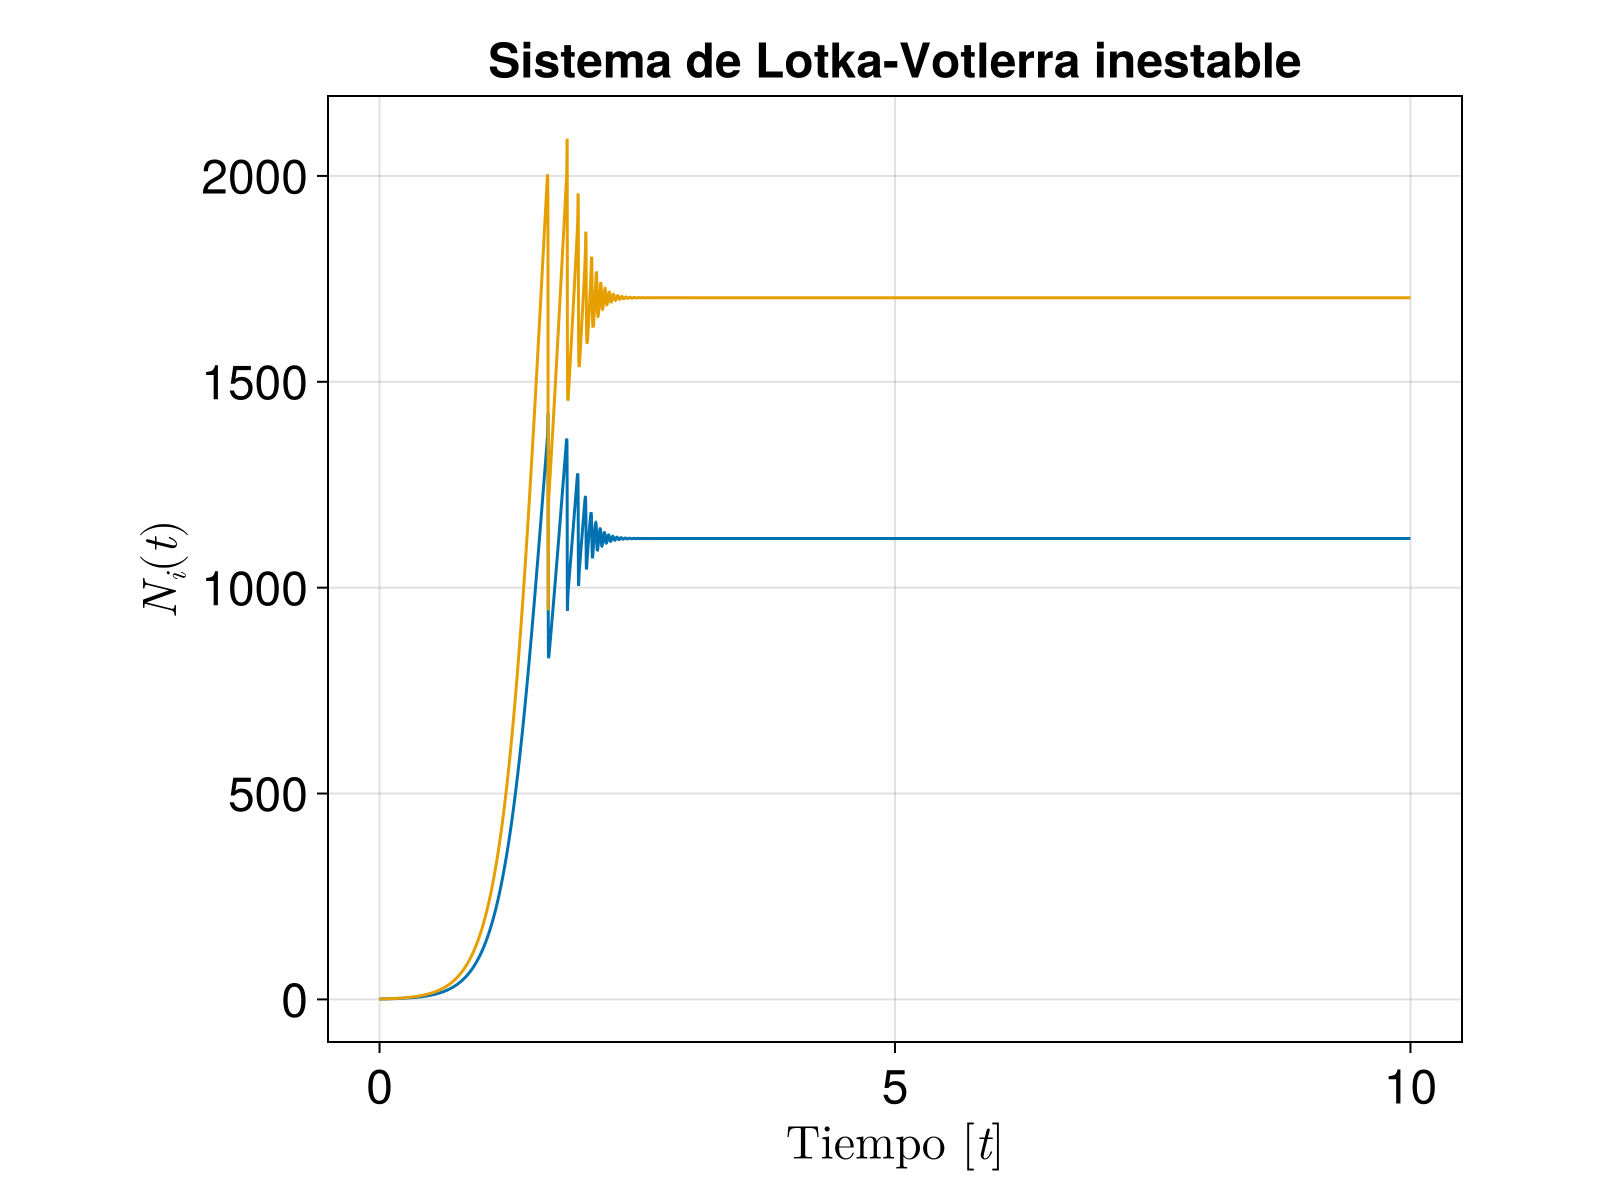
\includegraphics[scale=0.135]{../Imagenes/Heuristico2}
	\end{center}
	\vspace{-20pt} 
	\caption{Sistema marginalmente estable con interacciones $\alpha_{12}\alpha_{21}\approx 1$.}
	\vspace{-10pt}
	\label{fig:Heuristico2}
\end{wrapfigure}
En particular, cuando  $\alpha_{12}\alpha_{21}\approx 1$, el determinante se aproxima a cero y el sistema entra en un régimen de estabilidad marginal. En la Figura \eqref{fig:Heuristico2} se muestra una realización del sistema en la que el ciclo de interacción satisface $\alpha_{12}\alpha_{21}\approx 1$. En este régimen, las abundancias de equilibrio resultantes alcanzan valores varios órdenes de magnitud mayores que los observados en configuraciones alejadas del umbral de estabilidad. Asimismo, la dinámica exhibe oscilaciones transitorias antes de estabilizarse, lo que es característico de sistemas cercanos a la estabilidad marginal. Este ejemplo permite visualizar de manera directa el papel que desempeñan los ciclos de interacción de longitud dos en la organización del umbral de estabilidad. \\
\\
En sistemas de mayor dimensión, estos ciclos pueden interpretarse como contribuciones locales dentro de la red de interacciones. No obstante, su efecto no determina por sí mismo la estabilidad global del sistema, ya que en redes de mayor tamaño intervienen ciclos de interacción de orden superior que pueden modificar o compensar este mecanismo. Por esta razón, resulta conveniente considerar criterios estructurales más generales que permitan caracterizar la estabilidad del sistema en dimensiones mayores.

\subsection{Cono convexo}

Como se ha discutido anteriormente, la estabilidad ecológica está estrechamente relacionada con la factibilidad del estado de equilibrio, ya sea plena o parcial. No obstante, en general la factibilidad no implica la estabilidad del sistema, como ha sido ampliamente discutido en la literatura clásica \cite{goh1977feasibility}. En este sentido, la estabilidad dinámica depende adicionalmente de la estructura espectral de la matriz Jacobiana. Por esta razón, resulta de interés identificar condiciones estructurales que favorezcan la factibilidad del sistema y permitan restringir el análisis a configuraciones ecológicamente relevantes. En esta sección se introduce el marco geométrico del cono convexo para caracterizar la existencia de equilibrios factibles.\\
\\
Para este propósito se considera el equilibrio coexistente, definido por la relación $\Lambda X^*=\mathrm{K}$. Si el vector $\mathrm{K}$ esta contenido en el cono convexo generado por las columnas de $\Lambda$, entonces el equilibrio coexistente es factible. Para visualizar esta relación, se reescribe el producto matricial como una combinación lineal de los vectores columna de $\Lambda$,
$$\Lambda X^*=x_1^*\ell_1+x_2^*\ell_2+\cdots+x_n^*\ell_n$$

donde cada $\ell_i$ representa la $i$-ésima columna de la matriz $\Lambda$. De esta manera, el vector $\Lambda X^*$ se expresa como suma ponderada dichas columnas. El conjunto de todas las combinaciones lineales con coeficientes positivos define el cono convexo generado por $\Lambda$,
$$\operatorname{C}(\Lambda):=\left \{\sum_{i=1}^N  x_i\ell_i : x_i>0\right \}$$
Por lo tanto, el equilibrio coexistente es factible si y solo si $\mathrm{K}\in \operatorname{C}(\Lambda)$, lo que equivale a exigir $X^* > 0$. Cuando $\mathrm{K}$ se ubica en la frontera del cono, se tiene $x_i^*=0$ para al menos una especie, lo que corresponde a equilibrios parcialmente factibles. El análisis de estos casos requiere considerar subconjuntos de especies persistentes y las submatrices correspondientes de $\Lambda$, lo cual introduce una complejidad adicional. Por esta razón, en lo que sigue se centra la atención en el equilibrio de coexistencia. Finalmente, si $\mathrm{K}\notin \operatorname{C}(\Lambda)$, el equilibrio coexistente no es factible.

\subsubsection*{Diagonal dominante}

Una condición suficiente que favorece la factibilidad del estado coexistente consiste en imponer una diagonal dominante en la matriz de interacciones. Desde el punto de vista ecológico, esto implica que el término logístico asociado a la autorregulación de cada especie domina sobre la contribución interespecífica del sistema. En particular, debe cumplirse
$$\sum_{j\neq i}|\alpha_{ij}|<|\alpha_{ii}|$$
El lector recordará el \textit{criterio suficiente de estabilidad} presentado en la Proposición \ref{prop:DiagonalI}, el cual parte de la misma premisa \eqref{eqn:DesigualdadCoexistencia} para demostrar que los radios de Gershgorin permanecen contenidos en el semiplano negativo de $\mathbb{C}$. Desde esta perspectiva, la diagonal dominante no solo controla la localización espectral de la matriz Jacobiana, sino que también favorece la factibilidad del equilibrio.\\
\\
Geométricamente, esta condición induce un cono convexo que se extiende ampliamente dentro del primer ortante de $\mathbb{R}^n$, lo que incrementa la probabilidad de que el vector $\mathrm{K}$ pertenezca a $\operatorname{C}(\Lambda)$ y, por tanto, de que el equilibrio coexistente sea factible. En términos estadísticos, la condición necesaria para que esto ocurra recupera nuevamente el resultado
$$(N-1)p\sigma\sqrt{\frac{2}{\pi}}<1$$
En consecuencia, esta desigualdad implica simultáneamente que los discos de Gershgorin se mantengan contenidos en el semiplano negativo de $\mathbb{C}$ y que la factibilidad del equilibrio coexistente sea altamente probable. No obstante, este argumento se restringe al caso de coexistencia completa y no contempla los escenarios asociados a estados parcialmente factibles. Para extender esta caracterización se introduce a continuación un enfoque basado en una relación señal-ruido sobre la diagonal de la matriz de coeficientes de interacción $\Lambda$.

\subsubsection*{Relación Señal-Ruido}

Para extender el análisis anterior se introduce un criterio basado en una relación señal–ruido (SNR, por sus siglas en inglés). Este tipo de medida permite comparar la magnitud de un término dominante con respecto a las fluctuaciones que lo perturban. En el contexto de la matriz de interacciones $\Lambda$, esta relación puede interpretarse geométricamente como una medida de la desviación de los vectores columna $\ell_i$ con respecto a su eje coordenado correspondiente $\hat{e}_i$, desviación que surge a partir de las interacciones interespecíficas $\alpha_{ij}$ presentes en cada columna.\\
\\
De manera general, la relación señal–ruido se define como
$$\kappa = \frac{P_{\text{señal}}}{P_{\text{ruido}}}$$
En este caso, la señal se asocia con los elementos diagonales de $\Lambda$, que representan la autorregulación de cada especie, mientras que el ruido corresponde a las interacciones interespecíficas $\alpha_{ij}$. Desde esta perspectiva, la relación señal–ruido proporciona una medida efectiva de cuánto domina la contribución diagonal sobre las fluctuaciones inducidas por las interacciones del sistema.\\
\\
Bajo esta interpretación, el parámetro $\kappa$ puede utilizarse como un indicador estructural de la apertura del cono convexo generado por las columnas de $\Lambda$. En particular, valores grandes de $\kappa$ implican columnas cercanas a sus ejes coordenados, lo que favorece que el vector $\mathrm{K}$ quede contenido dentro de $\operatorname{C}(\Lambda)$ y, por consiguiente, la existencia de estados de equilibrio factibles.\\
\\
Dado que la abertura del cono convexo depende de las fluctuaciones inducidas por los términos $\alpha_{ij}$, los parámetros $\sigma$ y $p$ actúan como parámetros de control que determinan su geometría. Para cuantificar este efecto, considérese el producto interior entre un vector columna $\ell_i$ de $\Lambda$ y el vector $\mathrm{K}$
$$\ell_i^\top\cdot\mathrm{K}=\|\ell_i\|\|\mathrm{K}\|\cos\theta_i$$
donde $\theta_i$ es el ángulo entre ambos vectores. Para que la columna $\ell_i$ se abra en dirección de $\mathrm{K}$ se requiere idealmente que este producto sea positivo, lo cual equivale a $\cos\theta_i>0$. Al expandir el producto interior se obtiene
\begin{equation}\label{eqn:Señal-Ruido}
	\ell_i^\top\cdot\mathrm{K}
	= \sum_{j=1}^{N}\alpha_{ij}K_j.
\end{equation}
Considerando el caso homogéneo $K_j=K$, se tiene
$$\ell_i^\top\cdot\mathrm{K} = K\sum_{j=1}^{N}\alpha_{ij} = K\left(1+\sum_{j\neq i}\alpha_{ij}\right)$$
Cada elemento $\alpha_{ij}$ posee media cero y varianza $p\sigma^2$. Por lo tanto
$$
\mathbb{E}\!\left[\sum_{j\neq i}\alpha_{ij}\right]=0,
\qquad
\Var\!\left(\sum_{j\neq i}\alpha_{ij}\right)=(N-1)p\sigma^2
$$
Aplicando el teorema central del límite, la suma anterior se aproxima por una variable normal
$$
Y\sim\mathcal{N}\!\left(1,(N-1)p\sigma^2\right)
$$
Las fluctuaciones de esta distribución están gobernadas por la desviación estándar efectiva
$$
\sigma_{\text{eff}}=\sigma\sqrt{(N-1)p}
$$
lo que permite definir la relación señal–ruido como
\begin{equation}\label{eqn:SNR}
	\kappa=\frac{\mu}{\sigma_{\text{eff}}}
	=\frac{1}{\sigma\sqrt{(N-1)p}}.
\end{equation}
El objetivo es que la expresión (\ref{eqn:Señal-Ruido}) sea positiva, es decir, $Y>0$, lo cual garantiza que el vector columna $\ell_i$ se encuentre orientado en dirección de $\mathrm{K}$\footnote{Equivalente a que el ángulo entre ambos vectores satisfaga $|\theta|<\frac{\pi}{2}$.}. Dado que $Y$ es una variable aleatoria con distribución $Y\sim\mathcal{N}(\mu,\sigma_{\text{eff}}^2)$, lo que puede estimarse es la probabilidad de que esta condición se cumpla. Utilizando la función de distribución acumulada de la normal estándar se obtiene
\begin{align*}
	\text{Pr}(Y>0)
	&=\text{Pr}\left(Z>-\frac{\mu}{\sigma_{\text{eff}}}\right)\\
	&=1-\Phi\left(-\frac{\mu}{\sigma_{\text{eff}}}\right)\\
	&=\Phi\left(\frac{\mu}{\sigma_{\text{eff}}}\right),
\end{align*}
donde $\Phi(\cdot)$ denota la función de distribución acumulada de la normal estándar. En consecuencia, la probabilidad de que las columnas de $\Lambda$ se orienten en dirección de $\mathrm{K}$ queda determinada por la relación señal–ruido. Este resultado permite identificar configuraciones de la SNR que favorezcan la factibilidad del equilibrio y, por ende, sistemas de Lotka–Volterra estables con alta probabilidad. Asimismo, proporciona valores de $p$ y $\sigma$ que controlan dicha probabilidad en función de la estructura estadística de la matriz de interacciones. \\
\\
En el caso extremo $\sigma=1.0$, $p=1.0$ se obtiene
$$\kappa\approx  0.1005,\qquad \Phi(\kappa)\approx 0.54$$
Este resultado puede parecer contraintuitivo, ya que podría interpretarse erróneamente como una probabilidad del 54\% de que el sistema LV sea estable. Sin embargo, esta interpretación no es correcta. La cantidad $\Phi(\kappa)$ únicamente representa la probabilidad de que vector columna arbitrario $\ell_i\in\Lambda$ se encuentre alineado con la dirección del vector $\mathrm{K}$. En otras palabras, describe una propiedad local o marginal del conjunto de vectores columna de $\Lambda$, pero no proporciona información directa sobre la probabilidad de que el conjunto completo de vectores satisfaga simultáneamente la condición de alineación. \\
\\
Una posible forma de interpretar este resultado es pensar que, para un sistema con 
$N=100$, aproximadamente la mitad de los vectores columna presentan una orientación compatible con la dirección $\mathrm{K}$. No obstante, la factibilidad del sistema no depende de esta condición individual, sino de la geometría colectiva del cono convexo generado por todas las columnas de $\Lambda$. Incluso si una fracción significativa de vectores se encuentra aproximadamente alineada con $\mathrm{K}$, esto no garantiza que el cono convexo resultante se abra estrictamente en esa dirección ni que contenga al vector $\mathrm{K}$ en su interior\\
\\
Por lo tanto, se requiere que $\Phi(\kappa)$ tome valores suficientemente altos para que la mayoría de los vectores columna se orienten en la dirección de $\mathrm{K}$, favoreciendo así la formación de un cono convexo aproximadamente alineado con dicha dirección. Como criterio operativo se propone considerar valores de $\kappa$ cercanos a la unidad. En particular,
\begin{equation}\label{eqn:kappaEff}
	\kappa\approx 0.9,\qquad\Phi(\kappa)\approx 0.8159
\end{equation}
lo cual implica que un vector columna arbitrario de $\Lambda$ tiene aproximadamente un 
81.6\% de probabilidad de encontrarse orientado en la dirección de $\mathrm{K}$. Este umbral sugiere que la mayoría de los vectores columna contribuyen positivamente a la orientación del cono convexo en dicha dirección, incrementando así la probabilidad de que $\mathrm{K}$ quede contenido dentro del cono generado por $\Lambda$. Debe enfatizarse que esta condición no constituye un criterio estricto de estabilidad, sino un indicador estadístico que captura el grado promedio de alineamiento entre las columnas de $\Lambda$ y la dirección de $\mathrm{K}$.\\
\\
De la ecuación (\ref{eqn:SNR}) se obtiene una corrección del radio espectral asociada al alineamiento estadístico de las columnas de $\Lambda$ con la dirección de $\mathrm{K}$, lo cual favorece la abertura del cono convexo generado por $\Lambda$ en dicha dirección. Este efecto introduce un factor efectivo $\kappa$ en el criterio de estabilidad, de modo que
\begin{equation*}
	\begin{split}
		\kappa\sigma\sqrt{Np}<1
	\end{split},\qquad
	\begin{split}
		\sigma_c=\frac{1}{\kappa\sqrt{Np}},
	\end{split}\qquad\begin{split}
		p_c=\frac{1}{\kappa^2\sigma^2 N}
	\end{split}
\end{equation*}
considerando que $N\approx N-1$ cuando $N\gg 1$. Estas expresiones definen un umbral efectivo de estabilidad que incorpora el efecto geométrico del alineamiento estadístico entre las columnas de $\Lambda$ y la dirección de $\mathrm{K}$. En consecuencia, el parámetro $\kappa$ introduce una corrección al criterio clásico de estabilidad espectral, desplazando los valores críticos de $\sigma$ y $p$ que delimitan la transición entre estabilidad e inestabilidad en el sistema de Lotka–Volterra.

\section{Discusión}

\subsection{Sobre el carácter de la transición}

Existen trabajos que abordan modelo de Lotka-Volterra generalizado en términos de trasnciciones análogas a las observadas en sistemas de \textit{spin glasses}, como el trabajo de Guy Bunin \cite{bunin2017ecological}, donde se analiza la aparición de regímenes complejos en sistemas ecológicos de gran dimensión. En esta línea, distintos estudios ha explorado la posible existencia de fases críticas marginales del tipo Gardner, originalmente introducidas en la teoría de vidrios de spín \cite{biroli2018marginally,altieri2021properties}.
\\
\\
En particular, en el trabajo de Ada Altieri \textit{et al.} resulta relevante, ya que considera un modelo GLV con interacciones estrictamente simétricas y presencia de ruido estocástico.  Bajo esas condiciones, la dinámica puede reformularse como un flujo de gradiente asociado a un Hamiltoniano efectivo, de modo que el sistema evoluciona según. 
$$\frac{dx_i}{dt}=-\frac{\partial H}{\partial x_i}$$
En este contexto, el Hamiltoniano efectivo permite relacionar los mínimos de energía con los distintos atractores del sistema. El análisis estadístico de esta función de energía permite explorar distintos regímenes dinámicos conforme varían los parámetros del modelo. Dependiendo del régimen, el sistema puede presentar un único equilibrio estable, múltiples equilibrios o incluso un número exponencial de mínimos metaestables asociados a modos blandos característicos de la fase Gardner.
\\
\\
En este marco resulta particularmente útil analizar la matriz Hessiana del Hamiltoniano efectivo, denotada por $\mathcal{H}$, ya que su espectro caracteriza la estabilidad local de los puntos críticos del paisaje de energía. En particular, cuando todos los valores propios de la Hessiana son positivos
$$\lambda_{\min}>0$$
el punto crítico corresponde a un mínimo local del Hamiltoniano y, por tanto, a un atractor dinámico del sistema. En contraste, la aparición de valores propios que se aproximan a cero indica que la curvatura del paisaje de energía se aplana en ciertas direcciones, dando lugar a los denominados modos blandos asociados a estados de estabilidad marginal. Este fenómeno es característico de la fase crítica tipo Gardner, donde el número de mínimos metaestables puede crecer rápidamente con el tamaño del sistema. Finalmente, la presencia de valores propios negativos en la Hessiana indica direcciones inestables en el paisaje de energía, correspondientes a puntos silla o máximos del Hamiltoniano.
\newpage
En nuestro contexto se consideran sistemas de Lotka-Volterra generalizado con dinámica dirigida, de modo que la matriz de interacción no es simétrica, en general $\alpha_{ij}\neq\alpha_{ji}$. Bajo estas condiciones, la dinámica ya no puede escribirse como un flujo gradiente asociado a un potencial efectivo.  En particular, el campo vectorial del sistema no es conservativo, ya que las derivadas cruzadas no satisfacen la condición de integrabilidad
$$\frac{\partial f_i}{\partial x_j}\neq\frac{\partial f_j}{\partial x_i}$$
lo cual impide la definición de un Hamiltoniano global que describa la dinámica. En consecuencia, el análisis del sistema no puede formularse en términos de un paisaje de energía. En su lugar, la estabilidad del equilibrio se caracteriza a partir de la matriz Jacobiana evaluada en el equilibrio. De manera análoga al papel que desempeña la matriz Hessiana en sistemas tipo gradiente, el espectro de la Jacobiana determina la estabilidad lineal del equilibrio y permite identificar los regímenes dinámicos del sistema.\\
\\
Por esta razón, a lo largo de este trabajo se ha enfatizado que las transiciones observadas deben interpretarse como transiciones dinámicas, asociados a cambios de estabilidad del equilibrio, sin implicar la presencia de un mecanismo termodinámico subyacente ni una transición de fase en el sentido estadístico habitual.

\subsubsection*{Implicación ecológica}

Las distinción entre interacciones simétricas y asimétricas tiene implicaciones profundas para la naturaleza de la dinámica del sistema. Cuando la matriz de interacciones es simétrica, la dinámica del sistema puede reformularse como un flujo de gradiente asociado a un potencial efectivo. en este caso, el sistema satisface una condición análoga al balance detallado y su evolución puede interpretarse como un proceso de relajación hacia mínimos de un paisaje de energía efectivo.\\
\\
En contraste, cuando las interacciones son asimétricas, el campo vectorial deja de ser conservativo y ya no existe un potencial global que describa la dinámica. En términos dinámicos, esto implica la aparición de corrientes en el espacio de fases y la ausencia de una descripción en términos de un paisaje de energía. La asimetría de las interacciones introduce direccionalidad entre los intercambios entre especies y convierte al sistema en un ejemplo de sistema dinámico fuera de equilibrio, en el sentido de la teoría de sistemas disipativos desarrollada por Ilya Prigogine \cite{prigogine1963introduction}.
\\
\\
Desde una perspectiva ecológica, asumir interacciones estrictamente simétricas constituye un escenario altamente idealizado. Las interacciones entre especies suelen ser inherentemente dirigidas y heterogéneas, por lo que el modelo de Lotka-Volterra generalizado con interacciones no necesariamente simétricas proporciona una descripción más natural de ecosistemas como sistemas dinámicos fuera del equilibrio. En este contexto, las transiciones que observamos emergen de propiedades geométricas y espectrales de la matriz de interacción, particularmente de la organización de sus ciclos dirigidos y de las condiciones necesarias para la factibilidad del equilibrio.

\subsection{Sobre la simetría estructural}

En el contexto de la simetría estructural se introdujo previamente la condición \eqref{eqn:relacionHeuristica} como un criterio que garantiza estabilidad en el caso  $N=2$. En este escenario el sistema únicamente contiene un ciclo de interacción posible, correspondiente al par de interacciones recíprocas entre las especies. Como consecuencia, dicha condición controla de manera directa la estabilidad del equilibrio.\\
\\
Sin embargo, en sistemas de mayor dimensión $N\gg 1$ la situación cambia de manera cualitativa.  A medida que el número de especies aumenta, el sistema admite un número creciente de ciclos de interacción de orden superior. Estos ciclos contribuyen colectivamente a la estructura espectral de la matriz Jacobiana y, por lo tanto, a la estabilidad del equilibrio. En este régimen, los ciclos de interacción de orden dos dejan de ser el único mecanismo  relevante y su efecto queda inmerso dentro de una red mucho más compleja de retroalimentaciones dirigidas.\\
\\
En consecuencia, la estabilidad del sistema ya no puede entenderse únicamente a partir de condiciones locales a pares de especies, sino que emerge de la interacción global entre ciclos dirigidos de distintas longitudes. No obstante, la deformación observada en el espectro de $\Lambda$, y por consiguiente en el espectro de la matriz Jacobiana, puede estar relacionada con la presencia sistemática de ciclos de interacción de orden dos. La simetría estructural del soporte introduce correlaciones entre pares de entradas $\alpha_{ij}$ y $\alpha_{ji}$, asociadas a interacciones recíprocas entre especies. Estas correlaciones inducen simultáneamente componentes simétricas y antisimétricas en la matriz efectiva de interacción, lo que rompe la isotropía espectral característica de matrices completamente desordenadas. \\
\\
Como resultado, el espectro de $\Lambda$ tiende a elongarse preferencialmente en dirección de los ejes coordenados, en particular sobre el eje real. Este efecto modifica la localización del borde espectral de la Jacobiana y, por lo tanto, influye en las condiciones de estabilidad del equilibrio. En consecuencia, aunque los ciclos de interacción de orden dos no determinen por sí solos la estabilidad del sistema cuando $N\gg1$, sí introducen correlaciones estructurales que contribuyen a la deformación espectral observada.
\\
\\
Sin embargo, los resultados numéricos indican que la deformación del espectro no depende únicamente de la magnitud típica de las interacciones $\sigma$. En particular, se observan casos en redes altamente dispersas (ver Figura \eqref{fig:EspectroCoexistenteSim}) donde, aun para valores moderados de $\sigma$, el espectro presenta una deformación anisotrópica de tipo cruz. Esto sugiere que la estructura topológica de la red, y en particular el régimen de dispersión del soporte, puede amplificar el efecto de correlaciones locales asociadas a ciclos de interacción recíprocos. Por lo tanto, el papel preciso de los ciclos de interacción de orden dos en la organización espectral de la matriz $\Lambda$ requiere un análisis más detallado que excede el alcance del presente trabajo.

\subsection{Sobre la factibilidad y la estabilidad}

La estructura de la matriz de coeficientes de interacción $\Lambda$ determina la factibilidad del equilibrio, lo cual se ha analizado a lo largo de este trabajo mediante el marco geométrico del cono convexo generado por sus vectores columna. En este contexto, la factibilidad del equilibrio depende de que el vector de tasas intrínsecas pertenezca al cono convexo generado por dichas columnas.
\\
\\
Por otra parte, la estabilidad del equilibrio está gobernada por el espectro de la matriz Jacobiana del sistema. En el modelo de Lotka–Volterra generalizado, la Jacobiana puede escribirse como una transformación de $\Lambda$ ponderada por las abundancias del equilibrio $X^*$. En consecuencia, aunque las abundancias deformen la matriz efectiva del sistema, la organización global del espectro permanece fuertemente condicionada por la estructura de $\Lambda$.
\\
\\
En las simulaciones realizadas se consideraron matrices cuya distribución espectral presenta dos tipos de geometría principales: isotrópica y anisotrópica con elongación hacia los ejes coordenados. Sin embargo, no se exploraron deformaciones más extremas del espectro, por ejemplo configuraciones altamente elongadas hacia el eje real que podrían tener un impacto más directo en la estabilidad del equilibrio.
\\
\\
Bajo este marco, los resultados obtenidos sugieren que la estabilidad del sistema requiere necesariamente la existencia de un equilibrio factible —al menos parcialmente factible—, mientras que la factibilidad por sí misma no garantiza la estabilidad. En otras palabras, pueden existir equilibrios factibles cuya estructura espectral conduce a un equilibrio dinámicamente inestable.
\\
\\
La metodología utilizada en este trabajo se centró en identificar equilibrios estables a partir de las series de tiempo del sistema. Como consecuencia, el análisis no explora sistemáticamente el régimen en el cual existen estados factibles pero dinámicamente inestables. Este hecho resalta que, aun cuando el equilibrio sea factible desde el punto de vista geométrico, la organización espectral de $\Lambda$ ---y posteriormente de la matriz Jacobiana--- resulta determinante para establecer su estabilidad.
\\
\\
Finalmente, la geometría espectral de $\Lambda$ ---y en consecuencia de la matriz Jacobiana $\mathcal{J}$--- también determina la proximidad del sistema a la estabilidad marginal. En particular, cuando el espectro contiene valores propios que se aproximan a cero ($\lambda\to0$), el sistema desarrolla modos blandos asociados a tiempos de relajación largos, característicos de estados cercanos al umbral de estabilidad.

\subsection{Sobre el parámetro crítico}

El parámetro crítico propuesto en este trabajo se encuentra principalmente asociado a la factibilidad del estado equilibrio. Sin embargo, este parámetro no constituye por sí mismo un criterio estricto de estabilidad dinámica del equilibrio. En esta sección se propone un ajuste heurístico del parámetro crítico a partir de la observación de algunas transiciones dinámicas representativas. Este ajuste busca incorporar, de manera aproximada, el efecto que la estructura espectral del sistema tiene sobre la estabilidad. \\
\\
Resulta notable que la escala característica obtenida presenta la misma dependencia funcional que el parámetro clásico introducido por May para la estabilidad de sistemas ecológicos aleatorios. Esta coincidencia sugiere que ambas condiciones ---factibilidad y estabilidad--- pueden estar gobernadas por una misma escala estructural del sistema, aunque emergen de mecanismos conceptualmente distintos.
\\
\\
A continuación se presentan los valores del criterio suficiente de estabilidad y de la SNR ajustada a $\kappa=0.9$ para sistemas con soporte estructuralmente simétrico y dirigido. Ambos criterios se contrastan en sistemas dependientes de $p$ considerando los casos $\sigma=0.2$ y $\sigma=1.0$. En la Figura \eqref{fig:kappasigma02} se muestra el caso $\sigma=0.2$. El criterio suficiente de estabilidad delimita un régimen de conectividad $p$ donde el sistema permanece estable, cumpliendo su función como condición conservadora. En contraste, el valor crítico $p_c$ inducido por el parámetro 
$\kappa$ se ubica aproximadamente al inicio de la transición de estabilidad.
\begin{figure}[h!]
	\centering
	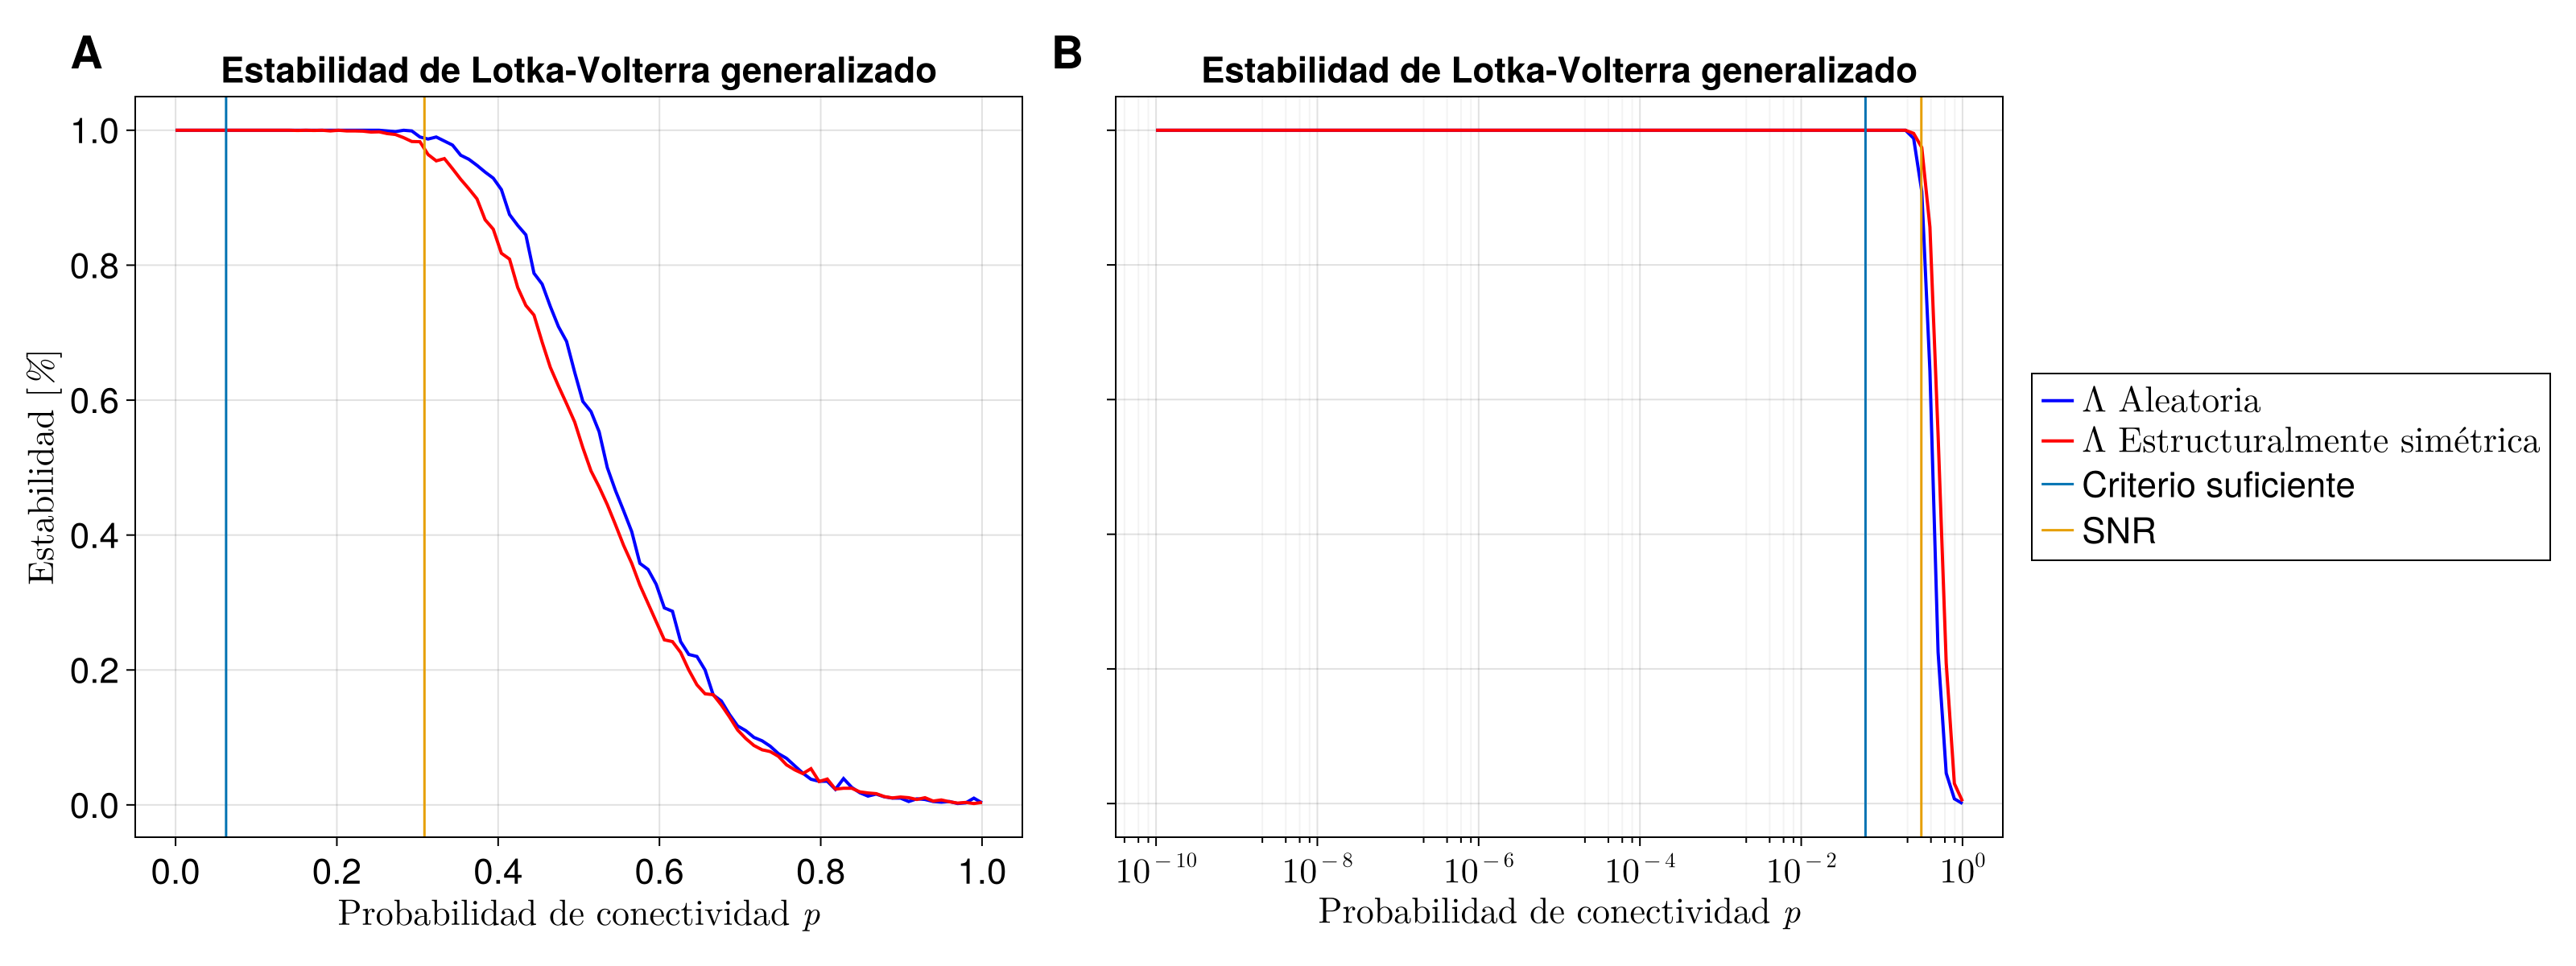
\includegraphics[scale=0.16]{../Imagenes/kappasigma02}
	\caption{Transición dinámica para $\sigma=0.2$ considerando $\kappa=0.9$. (\textbf{A}) Escala lineal. (\textbf{B}) Escala logarítmica.}
	\label{fig:kappasigma02}
\end{figure}

Debido a que en este escenario la transición ocurre a través de un transitorio amplio, el criterio basado en la SNR permite capturar de manera adecuada la separación entre un régimen estable, un régimen marginalmente estable asociado al transitorio dinámico, y finalmente un régimen inestable.\\
\\
Por otro lado, en la Figura \eqref{fig:kappasigma1} se muestra el contraste correspondiente al escenario $\sigma=1.0$. En este régimen ambos criterios se ubican en una escala de conectividad similar, describiendo adecuadamente la transición del sistema con soporte dirigido. En contraste, estos parámetros no reproducen de forma precisa la transición en el sistema con soporte estructuralmente simétrico. Incluso en este régimen persisten transitorios amplios que pueden atribuirse a la geometría espectral de las matrices $\Lambda$ y $\mathcal{J}$, particularmente a las deformaciones inducidas por las correlaciones asociadas a ciclos de interacción recíprocos.
\begin{figure}[h!]
	\centering
	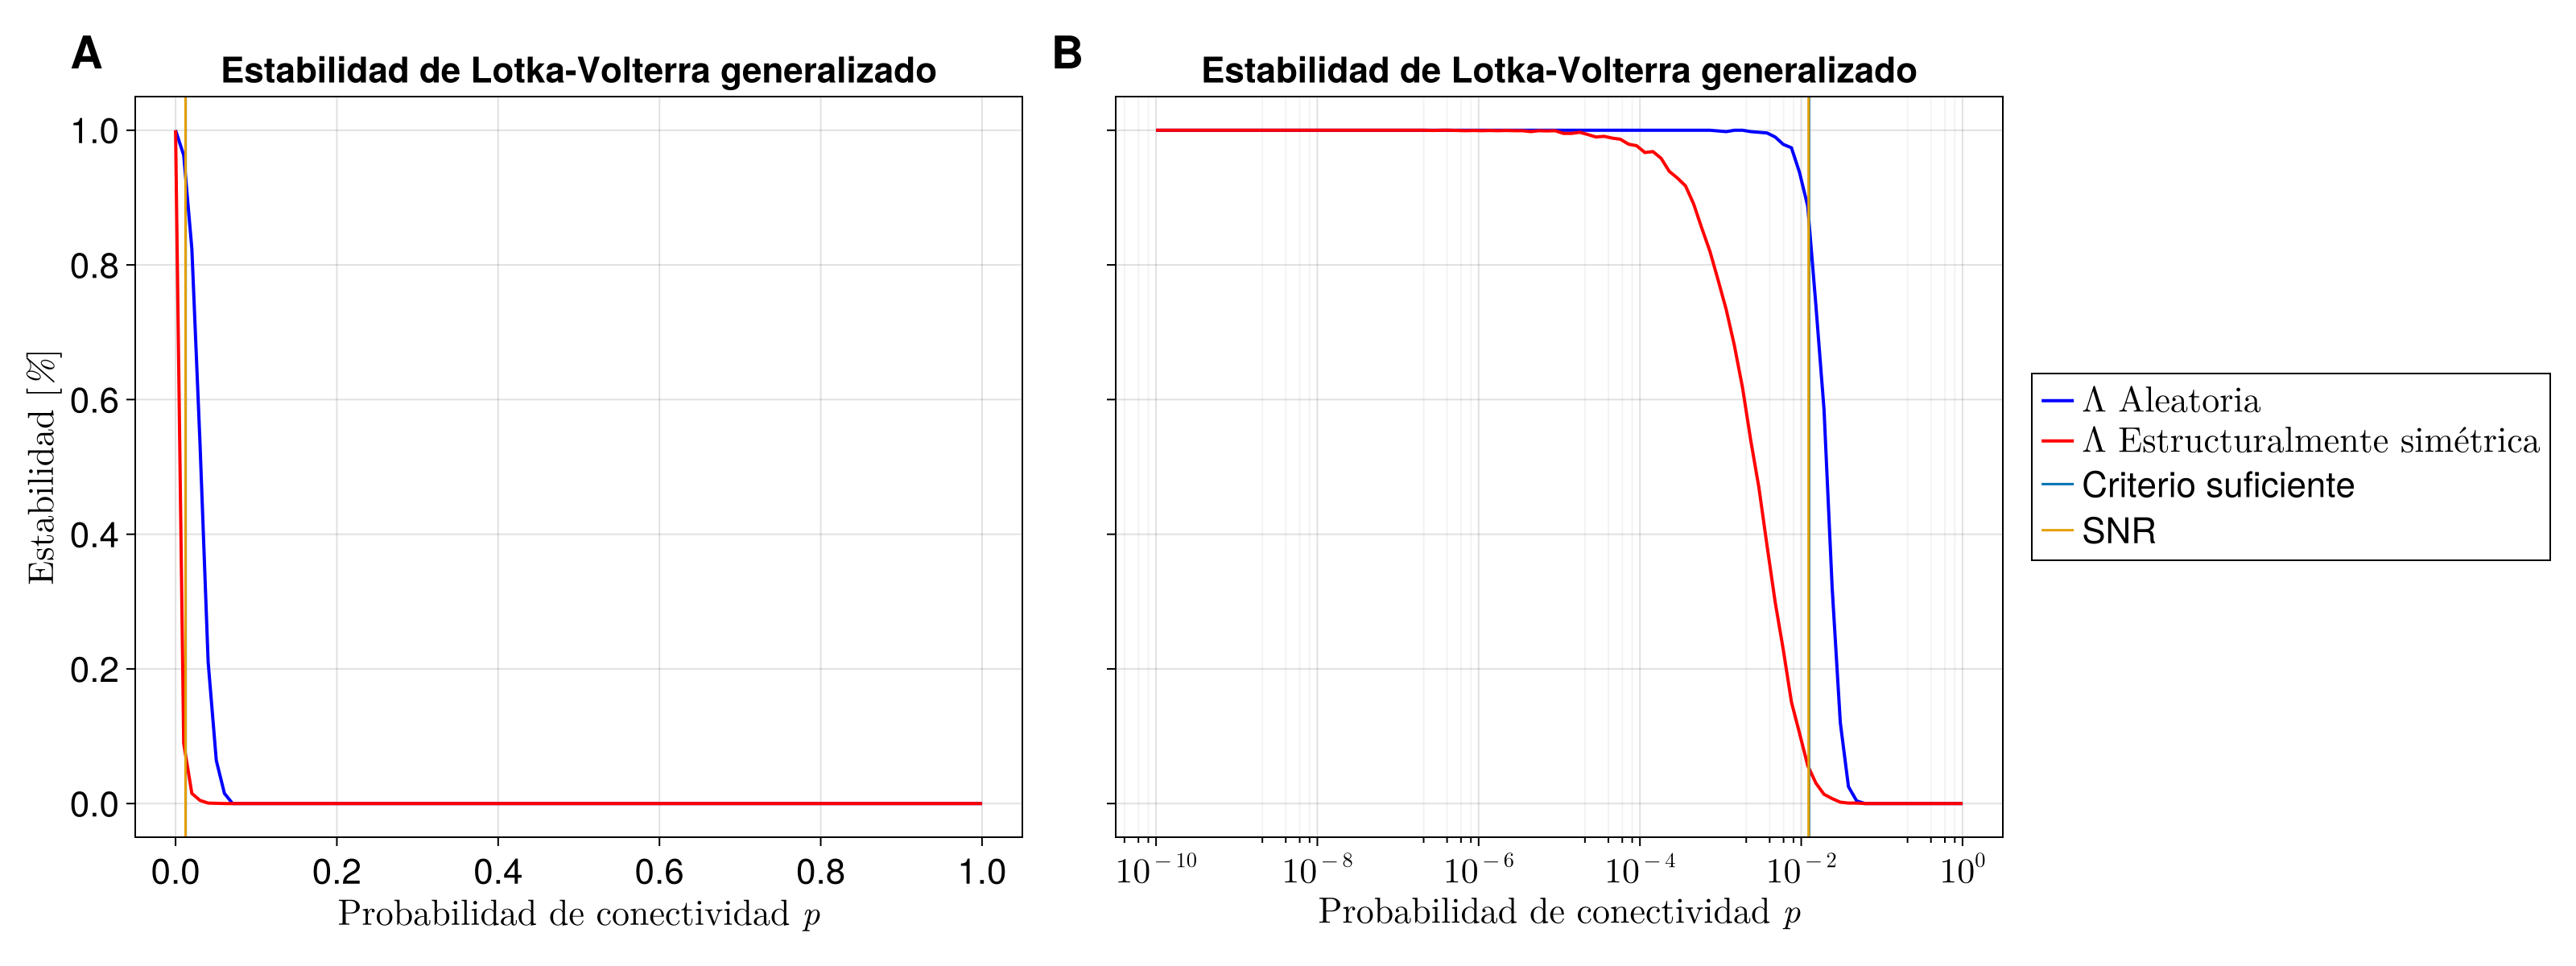
\includegraphics[scale=0.16]{../Imagenes/kappasigma1}
	\caption{Transición dinámica para el caso $\sigma=1.0$ considerando $\kappa=0.9$. (\textbf{A}) Escala lineal. (\textbf{B}) Escala logarítmica.}
	\label{fig:kappasigma1}
\end{figure}

En consecuencia, el caso estructuralmente simétrico requiere correcciones adicionales que incorporen de manera explícita estas correlaciones estructurales, lo cual queda fuera del alcance de esta tesis. En la Figura \eqref{fig:kappaps} se muestran dos transiciones en función de $\sigma$ para $p=0.1$ y $p=1.0$. En ambos casos se observa un comportamiento cualitativamente consistente con los resultados anteriores para el criterio suficiente de estabilidad y el parámetro basado en la SNR. Sin embargo, para $p=0.1$ se registran desviaciones entre los sistemas con soporte dirigido y con soporte estructuralmente simétrico. Estas diferencias pueden atribuirse a las correlaciones inducidas por la simetría estructural del soporte, las cuales modifican la geometría espectral de las matrices $\Lambda$ y $\mathcal{J}$\\
\\
En consecuencia, el valor crítico $\sigma_c$ inducido por el parámetro $\kappa$ también presenta desviaciones en el caso estructuralmente simétrico, lo que sugiere que este escenario requiere correcciones adicionales que incorporen explícitamente dichas correlaciones. Por lo tanto, el parámetro crítico propuesto debe entenderse como una construcción heurística que captura la escala característica del sistema. Aunque surge del análisis de la factibilidad del equilibrio, su dependencia funcional coincide con la escala que gobierna la expansión espectral de las matrices de interacción. Esta correspondencia sugiere la existencia de un puente conceptual entre la geometría de factibilidad y los criterios espectrales de estabilidad, cuya formalización rigurosa queda como una dirección natural para trabajos futuros.
\begin{figure}[t!]
	\centering
	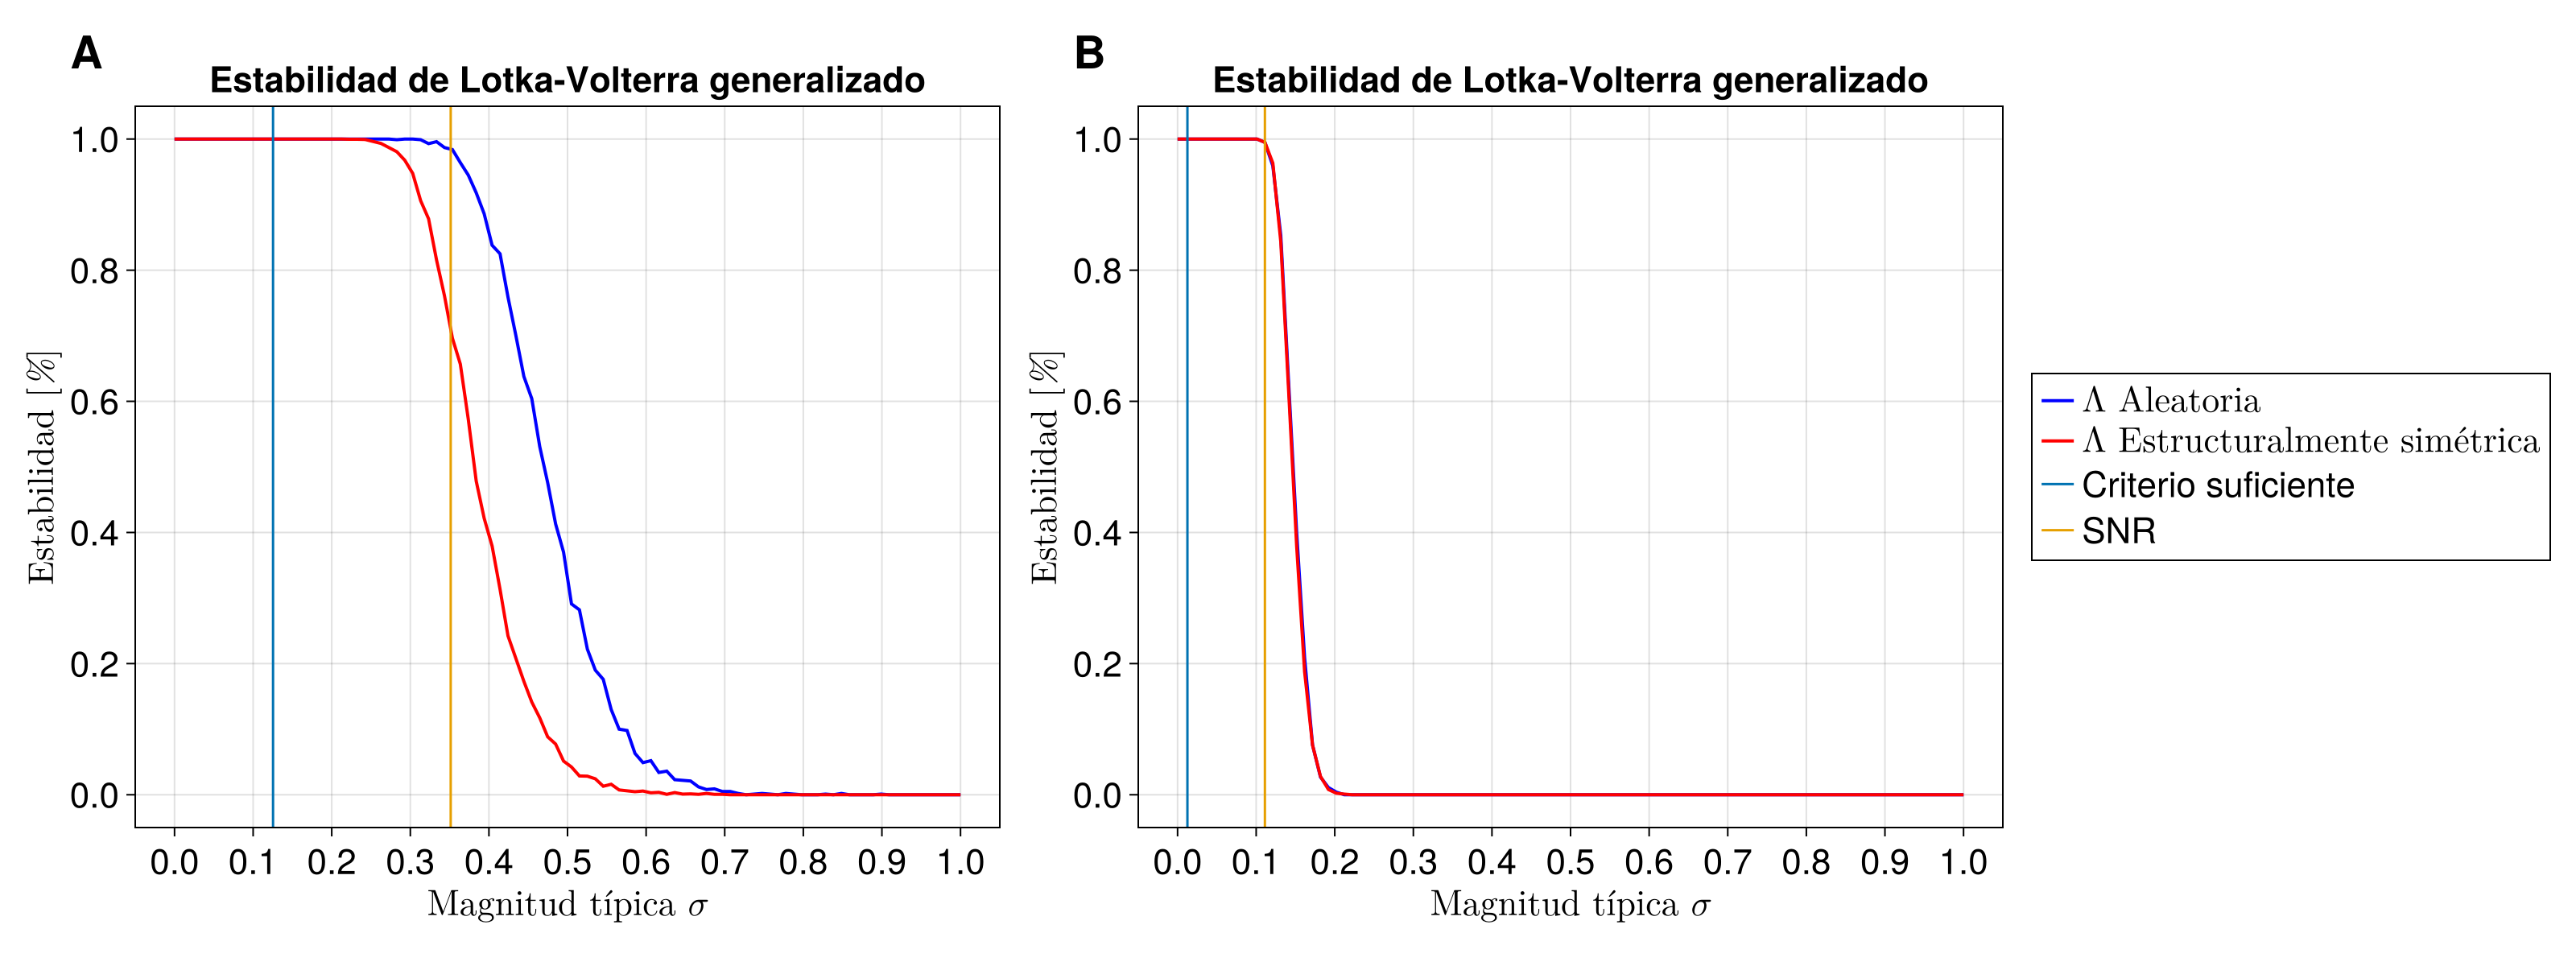
\includegraphics[scale=0.16]{../Imagenes/kappaps}
	\caption{Transiciones dinámica en función de $\sigma$ considerando $\kappa=0.9$. (\textbf{A}) Caso particular para $p=0.1$. (\textbf{B}) Caso particular para $p=1.0$.}
	\label{fig:kappaps}
\end{figure}

\subsection{Alcances y limitaciones}

El presente trabajo estudia sistemas de Lotka–Volterra generalizados en los cuales las interacciones entre especies se modelan mediante matrices aleatorias definidas sobre un soporte topológico. En particular, se consideran dos tipos de estructura de red: soportes dirigidos y estructuralmente simétricos, los cuales inducen diferentes patrones de correlación en las interacciones entre especies. La dinámica del sistema incorpora además un término de autorregulación logística que estabiliza el crecimiento individual de cada especie.
\\
\\
Dentro de este marco, el análisis se centra en la relación entre factibilidad del equilibrio y estabilidad dinámica. Para ello se utilizan herramientas provenientes de la geometría convexa, que permiten caracterizar la factibilidad de los estados estacionarios, y del análisis espectral de matrices aleatorias, que describe la estabilidad del sistema a partir de la distribución de valores propios de la matriz Jacobiana. Este enfoque permite identificar cómo la estructura estadística de la matriz de interacciones y la topología del soporte influyen en la geometría espectral del sistema y, en consecuencia, en su estabilidad.
\\
\\
Los resultados obtenidos se interpretan en el contexto de sistemas de gran dimensión y con interacciones aleatorias, donde la estructura espectral de las matrices de interacción presenta distribuciones aproximadamente isotrópicas o deformaciones moderadas inducidas por correlaciones estructurales del soporte. En particular, el trabajo explora cómo estas correlaciones pueden modificar la geometría del espectro y afectar las condiciones de estabilidad del equilibrio.
\\
\\
No obstante, el alcance del estudio presenta ciertas limitaciones. La metodología empleada se enfocó en sistemas cuya dinámica converge hacia un equilibrio estable, lo cual permitió identificar los puntos fijos a partir de simulaciones dinámicas. Como consecuencia, no se investigó de manera sistemática el régimen en el que existen equilibrios factibles pero dinámicamente inestables, ni se exploraron otros comportamientos dinámicos posibles como ciclos límite o dinámicas no estacionarias. Asimismo, el análisis se restringe a redes aleatorias simples y no considera estructuras de interacción más complejas que podrían surgir en sistemas ecológicos reales.


%\subfile{./TeX_files/AuxiliarComp.tex}

